% PAKETE UND DOKUMENTKONFIGURATION
\documentclass[11pt, a4paper]{article}

% Encoding für Umlaute
\usepackage[utf8]{inputenc}
\usepackage[T1]{fontenc}

% Silbentrennung
\usepackage[ngerman]{babel}

% erweiterte Matheumgebungen und Formelnummer mit Sectionnummer
\usepackage{amsmath}
\numberwithin{equation}{section}

% Braket Notation
\usepackage{braket}
\usepackage{isotope}
\usepackage[version=3]{mhchem}
\usepackage{tensor}
\usepackage{slashed}

% zusätzliche mathematische Schriftarten
\usepackage{amsfonts}

% verschiedene mathematische Symbole
\usepackage{amssymb}

% Einheiten setzen z.B. \SI{10}{\kilo\gram\meter\per\second\squared}
% Fehler: \SI{10 +- 0,2e-4}{\metre}
\usepackage{siunitx}
\sisetup{
  output-decimal-marker={,},
  separate-uncertainty
}

% Einheitendefinitionen
\DeclareSIUnit{\skt}{Skt.}
\DeclareSIUnit{\gauss}{G}
\DeclareSIUnit{\division}{div.}

% Operatordefinitionen
\DeclareMathOperator{\erf}{erf}

% Randbreiten
\usepackage[left=3.5cm,right=3.5cm,top=3cm,bottom=3cm,twoside]{geometry}

% Bilder einfügen
\usepackage{graphicx}
\usepackage[percent]{overpic}

% Textfarbe
\usepackage{color}

% Verweise innerhalb des Dokuments
\usepackage{hyperref}
\hypersetup{
	colorlinks = true,
	allcolors = {black}
}

% bessere Tabellenlayouts
\usepackage{booktabs}
\usepackage{multirow}
\usepackage{multicol}

% Seitenlayout (Kopfzeile)
\usepackage{fancyhdr}

% Float Barriers
\usepackage{placeins}

% Pakete für gedrehte Subfigures
\usepackage{caption}
\usepackage{subcaption}
\usepackage{rotating}

% Paket für textumflossene Abbildungen und Tabellen
\usepackage{wrapfig}

\usepackage{float}

% Caption-Setup
\captionsetup{font={small}}
\renewcommand{\thefigure}{\thesection.\arabic{figure}}
\renewcommand{\thesubfigure}{\alph{subfigure}}
\renewcommand{\thetable}{\thesection.\arabic{table}}
\renewcommand{\thesubtable}{\alph{subtable}}

% Manuelle Silbentrennung
\hyphenation{Par-ton-ver-teil-ungs-funk-tio-nen}

% Tiefe des Inhaltsverzeichnisses (Level: 1 sections, 2 subsections,
% 3 subsubsections)
\setcounter{tocdepth}{3}

% Code Einbettung
\usepackage{listings}
\definecolor{dkgreen}{rgb}{0,0.6,0}
\definecolor{gray}{rgb}{0.5,0.5,0.5}
\definecolor{mauve}{rgb}{0.58,0,0.82}

\lstset{frame=tb,
	aboveskip=3mm,
	belowskip=3mm,
	showstringspaces=false,
	columns=flexible,
	basicstyle={\ttfamily},
	numbers=left,
	numbersep=4pt,
	numberstyle=\tiny\color{black},
	keywordstyle=\color{blue},
	commentstyle=\color{dkgreen},
	stringstyle=\color{mauve},
	breaklines=true,
	breakatwhitespace=true,
	tabsize=3,
	xleftmargin=1em,
	xrightmargin=0.8em
}

% FANCYHDR SETUP
\pagestyle{fancy}
\fancyhead[EL,OR]{\thepage}
\fancyhead[ER]{\leftmark}
\fancyhead[OL]{\rightmark}
\setlength{\headheight}{13.6pt}

\renewcommand{\sectionmark}[1]{
\markboth{\thesection{} #1}{\thesection{} #1}
}
\renewcommand{\subsectionmark}[1]{
\markright{\thesubsection{} #1}
}

\newcommand{\korr}[1]{{\color{red}(#1)}}

% DOKUMENTINFORMATIONEN
\title{E214 \\ ATLAS}

\author{Christopher Deutsch\footnote{christopher.deutsch@uni-bonn.de} \and Christian Bespin\footnote{christian.bespin@uni-bonn.de}}

\date{\today}

\begin{document}

\begin{titlepage}

\maketitle

% DURCHFÜHRUNGSDATUM UND TUTOR
\begin{center}
\begin{tabular}{l r}
Durchführung: & 7./8. März 2016 \\
Gruppe: & P8 \\
Tutor: & Elisabeth Schopf
\end{tabular}
\end{center}

% ZUSAMMENFASSUNG
\begin{abstract}
\noindent In diesem Praktikumsversuch sollen Ereignisse am ATLAS Detektor am LHC untersucht werden.
Es wird die Detektorantwort auf verschiedene Teilchen analysiert und das elektromagnetische Kalorimeters kalibriert, um im Anschluss die Masse des W-Bosons zu bestimmen.
\end{abstract}

\end{titlepage}

% INHALTSVERZEICHNIS
\tableofcontents
% Neue Seite nach TOC
\newpage

% INHALT VERSUCHSPROTOKOLL
\section{Theorie}

\subsection{Einführung}

\subsubsection{Standardmodell}

Das Standardmodell beschreibt die Elementarteilchen und die Wechselwirkungen zwischen ihnen, mit Ausnahme der Gravitation und vereint somit die Erkenntnisse der Teilchenphysik.
Es gilt seit der Entdeckung des Higgs-Bosons als abgeschlossen.
Im Rahmen des Standardmodells können die einzelnen Elementarteilchen in Gruppen zu Leptonen, Quarks und Kraftteilchen zusammengefasst werden.
Leptonen und Quarks sind Fermionen, d.h. sie sind Spin~-$1/2$-Teilchen und unterscheiden sich durch ihre Ladung.
Während Leptonen, deren bekanntester Vertreter das Elektron ist, eine Ladungszahl~$1$ haben und die zugehörigen Neutrinos ungeladen sind, tragen Quarks drittelzahlige Ladungen~($1/3$ bzw.~$2/3$).
Durch Eichbosonen, wie Photon, Gluon, Z- und W-Boson wirken Kräfte zwischen den Quarks und Leptonen.
Das Higgs-Boson fällt aus dieser Einteilung heraus, da es eine Folge der spontanen Symmetriebrechung ist, die mit der Ursache von Masse assoziiert wird.

Durch diese Einteilung lässt sich eine Übersicht der einzelnen Elementarteilchen des Standardmodells gut wie in Abbildung \ref{fig:standardmodell} grafisch darstellen.
\begin{figure}[htbp]
	\centering
	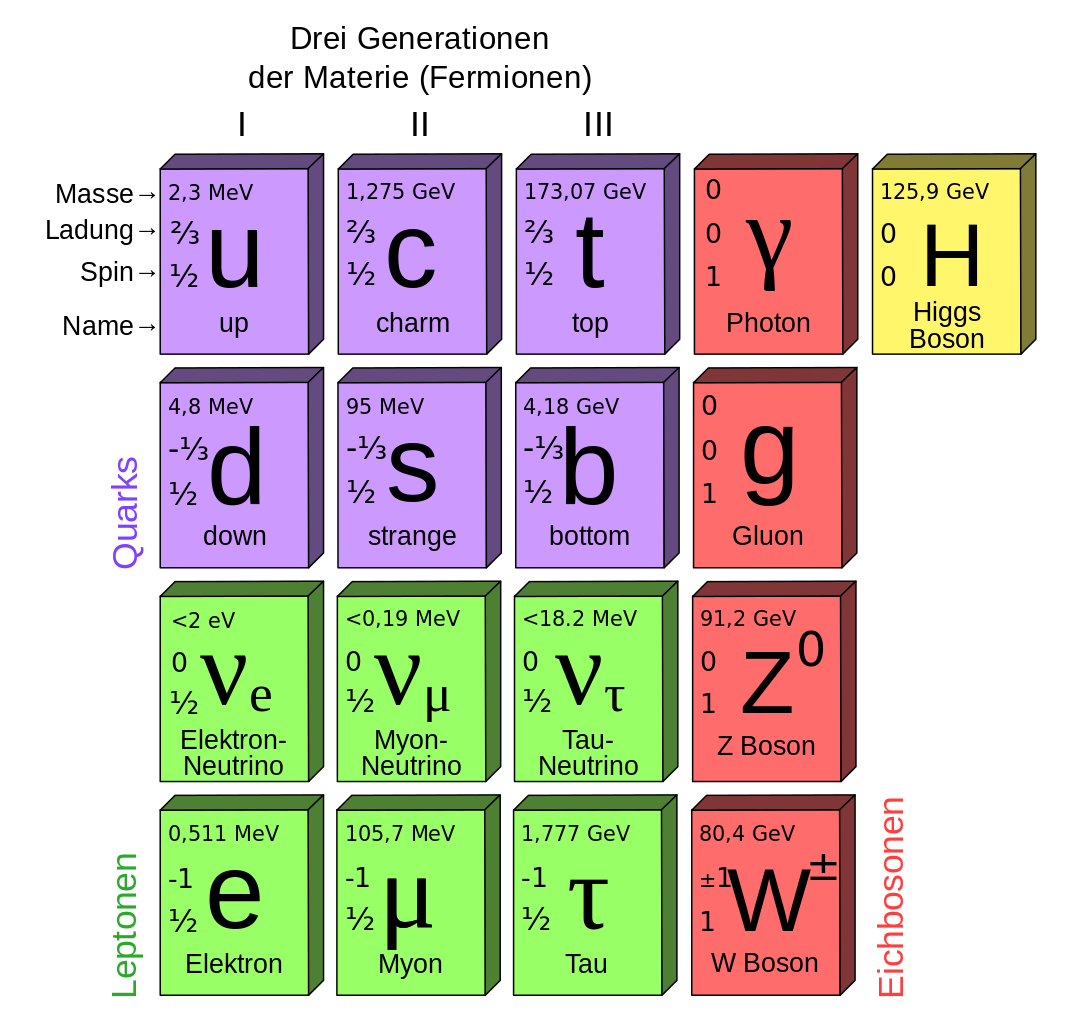
\includegraphics[width=.6\textwidth]{./figures/standardmodell}
	\caption{Standardmodell der Elementarteilchenphysik (aus \cite{wiki_standardmodell}).}
	\label{fig:standardmodell}
\end{figure}

\subsubsection{LHC und ATLAS}

Der Large Hadron Collider (LHC) der europäischen Organisation für Kernforschung (CERN) ist der zur Zeit weltgrößte Teilchenbeschleuniger mit einer Schwerpunktsenergie von bis zu~\SI{14}{TeV}.
Dadurch können physikalische Hypothesen bei hohen Energien überprüft und möglicherweise neue Beobachtungen gemacht werden.
Hierzu kommen vier Detektoren zum Einsatz, von denen zwei der Untersuchung hochenergetischer Ereignisse auf der Tera-Skala dienen.
Einer dieser Detektoren ist der ATLAS-Detektor, mit dem die in diesem Versuch analysierten Daten aufgenommen wurden.
In Abbildung \ref{fig:atlas} ist der ATLAS Detektor gezeigt.
\begin{figure}[htbp]
	\centering
	\includegraphics[width=\textwidth]{./figures/atlas}
	\caption{ATLAS Detektor\cite{cern}}
	\label{fig:atlas}
\end{figure}
In der Mitte des Bildes sind in rot die Pixeldetektoren und Siliziumdetektoren zur Spurrekonstruktion geladener Teilchen zu sehen.
Mit wachsendem Abstand zum Interaktionspunkt folgen die Übergangsstrahlungsdetektoren, die ebenfalls zur Rekonstruktion von Spuren geladener Teilchen genutzt werden.
Diese sind in der Grafik gelb dargestellt.
In braun und grün schließen sich die Kalorimeter an, wobei das innere zur Energiemessung elektromagnetisch wechselwirkender Teilchen konzipiert ist, während das äußere Kalorimeter, das Hadronenkalorimeter für schwere Teilchen geeignet ist.
Beide Kalorimeter bestehen aus vielen Modulen, die so dimensioniert sind, dass die jeweiligen Teilchen in ihnen gestoppt werden, um eine möglichst optimale Energiemessung durchzuführen.
Der gesamte Detektor wird dabei von einem Magnetfeld durchsetzt, das die Trajektorien geladener Teilchen krümmt, so dass aus der Krümmung der Impuls dieser bestimmt werden kann.

Um den s.g. inneren Detektor und die Kalorimeter liegt das Myonsystem, welches den äußeren Detektor bildet und allein der Detektion von Myonen dient.
Es ist in Abbildung \ref{fig:atlas} blau dargestellt.
Das Myonsystem beinhaltet wie der innere Detektor Elemente zur Spurrekonstruktion und Impulsmessung.


\subsection{Kinematik}

\subsubsection{Lorentzvektoren}
Ein Lorentzvektor~$\mathbf{x}$ ist ein vierdimensionaler Vektor mit reellen Komponenten, welche bezüglich einer Lorentztransformation~$\Lambda$ gemäß
\begin{align*}
	{x^\prime}^\mu = \tensor{\Lambda}{^\mu_\nu} x^\nu \qquad {x^\prime}_\mu = \tensor{\left(\Lambda^{-1}\right)}{^\nu_\mu} x_\nu
\end{align*}
transformieren.
Dadurch ist das Minkowski-Produkt zweier Lorentzvektoren
\begin{align*}
	\mathbf{x} \cdot \mathbf{y} = \tensor{g}{_\mu_\nu} x^\mu y^\nu \quad \text{mit} \quad g = \mathrm{diag}(1,-1,-1,-1)
\end{align*}
invariant unter Lorentztransformationen.

Ein solcher Lorentzvektor ist der sog.\ Viererimpuls~$\mathbf{p} = \left(E, \vec{p}\right)$, bestehend aus der Gesamtenergie~$E$ und dem Impuls~$\vec{p}$ im jeweiligen Bezugssystem.
Dieser ist essenziell für kinematische Betrachtungen in der Teilchenphysik und tritt häufig in Form von lorentzinvarianten Skalarprodukten auf, die in einem beliebigen Bezugssystem (z.B.\ im Schwerpunktssystem) ausgewertet werden können.

Beispiele dafür sind die invariante Masse eines Teilchens~$m_\mathrm{inv}^2 = \mathbf{p}^2$ oder die Mandelstam-Variable~$s = (\mathbf{p_1} + \mathbf{p_2})^2$, welche der quadratischen Schwerpunktsenergie zweier Teilchen entspricht.

\subsubsection{Rapidität und Pseudorapidität}
Die Rapidität entlang der Strahlachse~$z$ eines Teilchenbeschleunigers ist definiert als
\begin{align*}
	y = \frac{1}{2}\ln\left( \frac{E+p_z}{E-p_z} \right)
\end{align*}
mit der Energie~$E$ und dem Impuls~$p_z$ entlang der Strahlachse.
Wie das Lorentz-Beta~$\beta$ ist die Rapidität ein Maß für die Geschwindigkeit eines Teilchens.
Jedoch ist die Rapidität im Vergleich zu $\beta$ gegenüber Lorentz-Boosts entlang der Strahlachse lorentzinvariant und somit ein additives Geschwindigkeitsmaß, wie es bereits aus der klassischen Mechanik bekannt ist.

Für Teilchen mit verschwindender Masse ($E \approx p$) geht die Rapidität~$y$ in die Pseudorapidität~$\eta$ über
\begin{align}
	\eta = \frac{1}{2} \ln\left( \frac{1 + \cos\theta}{1 - \cos\theta} \right) = - \ln\left( \tan\frac{\theta}{2} \right)\text{,}
	\label{eq:pseudorapidity}
\end{align}
welche nur noch eine Funktion des Polarwinkels $\theta$ im jeweiligen Bezugssystem darstellt.
Im Gegensatz zu dem Polarwinkel~$\theta$ sind Pseudorapiditätsdifferenzen lorentzinvariant und somit ein bevorzugtes Maß für die Beschreibung von Ereignissen in Teilchendetektoren.
Beispielsweise eine Pseudorapidität von $\eta = \num{0}$ einem Polarwinkel von $\theta = \SI{90}{\degree}$ (senkrecht zur Strahlachse) und positive/negative Pseudorapiditäten entsprechen Winkeln in/entgegen der Richtung der Strahlachse.

\subsubsection{Hadronen-Kollision}
\label{sssec:hadronen_kollision}
Bei Kollisionen an Hadronenbeschleunigern wie dem LHC gilt es zu beachten, dass die eigentliche Kollision nicht zwischen den Hadronen, sondern dessen Partonen stattfindet.
Im Partonmodell besteht jedes Hadron neben Valenzquarks auch aus Gluonen und paarerzeugten Quark-Antiquark-Paaren.
Jedes Parton trägt dabei einen Impulsbruchteil, welcher im Bezugssystem in dem das Hadron einen unendlichen longitudinalen Impuls hat (d.h.\ transversale Impulse können vernachlässigt werden) durch die Bjorken'sche Skalenvariable~$x$ gegeben ist.

Zur Charakterisierung von Hadronen-Kollisionen ist es demnach erforderlich die Wahrscheinlichkeitsverteilung, dass ein Parton den Impulsbruchteil~$x$ des Hadrons trägt, zu bestimmen.
Diese Verteilungen, welche man Partonverteilungsfunktionen~$f(x)$ nennt, wurden für die verschiedenen Partonentypen~($u, \bar{u}, d, \dots, g$) an mehreren Teilchenbeschleunigern vermessen.

Dennoch sind die spezifischen Impulsbruchteile~$x_1, x_2$ der kollidierenden Partonen in der Regel unbekannt, so dass der Transversalimpuls~$p_\mathrm{T}$, welcher beispielsweise im durch den Krümmungsradius geladener Teilchen im äußeren Magnetfeld bestimmt werden kann, für die Auswertung herangezogen wird.
Darüber hinaus kann aus der Summe der Transversalimpulse aller Teilchen im Endzustand, welche gemäß der Impulserhaltung für frontal zusammenstoßende Partonen zu null summieren müssen, fehlender Transversalimpuls reproduziert werden, der auf nicht-detektierbare Teilchen wie Neutrinos zurückzuführen ist.

Da der Transversalimpuls für ungeladene Teilchen wie beispielsweise Photonen nicht durch den Krümmungsradius im Magnetfeld vermessen werden kann, wird stattdessen auf die Energieeinträge in den Kalorimetern zurückgegriffen und die Größe der fehlenden transversalen Energie~$\slashed{E}_\mathrm{T}$
\begin{align*}
	\slashed{E}_\mathrm{T} = - \sum_{i} E^i \sin\theta_i \, \vec{n}_{i,\perp}
\end{align*}
mit den Energieeinträgen~$E_i$ des Kalorimeters unter Polarwinkeln~$\theta_i$  und azimuthalen Einheitsvektoren~$\vec{n}_{i,\perp}$ auf den jeweiligen Eintrag, definiert.

\subsubsection{Kinematik des Zweikörperzerfalls}
\label{sssec:kinamtik_zweikoerperzerfall}
In diesem Versuch sollen Zerfälle von W und Z-Bosonen der Form 
\begin{align*}
	W &\rightarrow \ell + \nu \\
	Z^0 &\rightarrow \ell^- + \ell^+
\end{align*}
untersucht werden.
Um aus solchen Zerfällen Informationen gewinnen zu können, ist es nötig die Kinematik von Zweikörperzerfällen zu betrachten.
Aufgrund von Impulserhaltung haben die Tochterteilchen im Schwerpunktsystem (Ruhesystem des Mutterteilchens) betraglich gleiche aber antiparallele Impulse.
Das Ziel ist, eine Aussage über die Kinematik des Zerfalls zu machen, indem lediglich eins der Tochterteilchen des Zerfalls im Versuch gemessen wird (das Neutrino im W-Zerfall ist nur durch fehlende Energie zu detektieren).
Eine Schwierigkeit stellen die in diesem Versuch betrachteten Hadronen-Kollisionen gemäß Abschnitt~\ref{sssec:hadronen_kollision} dar, die keine Aussage über den longitudinalen Impuls der Tochterteilchen erlauben.
Stattdessen kann der transversale Impuls~$p_\mathrm{T}$ eines der Tochterteilchen für die Beschreibung verwendet werden.
An dieser Stelle wurde jedoch das Koordinatensystem der Betrachtung explizit gewählt (Ruhesystem des Mutterteilchens).
Das Spektrum des transversalen Impulses~$p_\mathrm{T}$ für eines der Tochterteilchen lässt sich mithilfe einer Jakobi-Transformation als \cite{script}:
\begin{align}
	\label{eq:pt_spektrum}
	\frac{\mathrm{d} \sigma}{\mathrm{d}p_\mathrm{T}} = \frac{\mathrm{d}\sigma}{\mathrm{d}\cos\vartheta^*} \frac{2 p_\mathrm{T}}{M} \frac{1}{\sqrt{\frac{1}{4} M^2 - p_\mathrm{T}^2}}
\end{align}
schreiben (vgl.\ Abschnitt \ref{sssec:herleitung_jacobi} für die Herleitung).
Man sieht, dass das transversale Impulsspektrum eine Polstelle bei der halben Masse des Mutterkerns~$M$ aufweist, welche zur Massebestimmung genutzt werden kann.
Dabei gilt es zu beachten, dass eine Abweichung vom gewählten Koordinatensystem (d.h.\ ein nicht-ruhendes Mutterteilchen) zu einer Verbreiterung der Polstelle in Gleichung \eqref{eq:pt_spektrum} führt.

\section{Beschreibung der verwendeten Software}

\subsection{Atlantis}

Zur Darstellung von Ereignissen wird das Programm Atlantis verwendet, das den Aufbau des ATLAS Detektors zeigt und die jeweiligen Signale der einzelnen Subdetektoren für einzelne Ereignisse darstellt.
Das Hauptfenster ist dabei in vier Darstellungen geteilt, wie in Abbildung \ref{fig:atlantis} zu sehen ist.
Den größten Bildbereich nimmt eine Ansicht der $xy$-Ebene des Detektors ein, die den gesamten Querschnitt zeigt.
Zusätzlich wird oben rechts ebenfalls eine Ansicht des Querschnitts gezeigt, jedoch mit Fokus auf den inneren Detektor, in dem Trajektorien geladener Teilchen dargestellt werden können. Am rechten Rand des Fensters ist ein Schnitt des Detektors in Längstrichtung gezeigt, während im unteren Bereich eine Ausschnitt in dieser $\rho z$-Ebene gezeigt wird, der vor allem den Bereich des inneren Detektors und der Kalorimeter zeigt, aber das Myonsystem ausblendet.
Die Anzahl und Ansicht der einzelnen Fenster kann dabei individuell geändert werden je nach Information, die man aus einem Ereignis gewinnen möchte.
\begin{figure}[htbp]
	\centering
	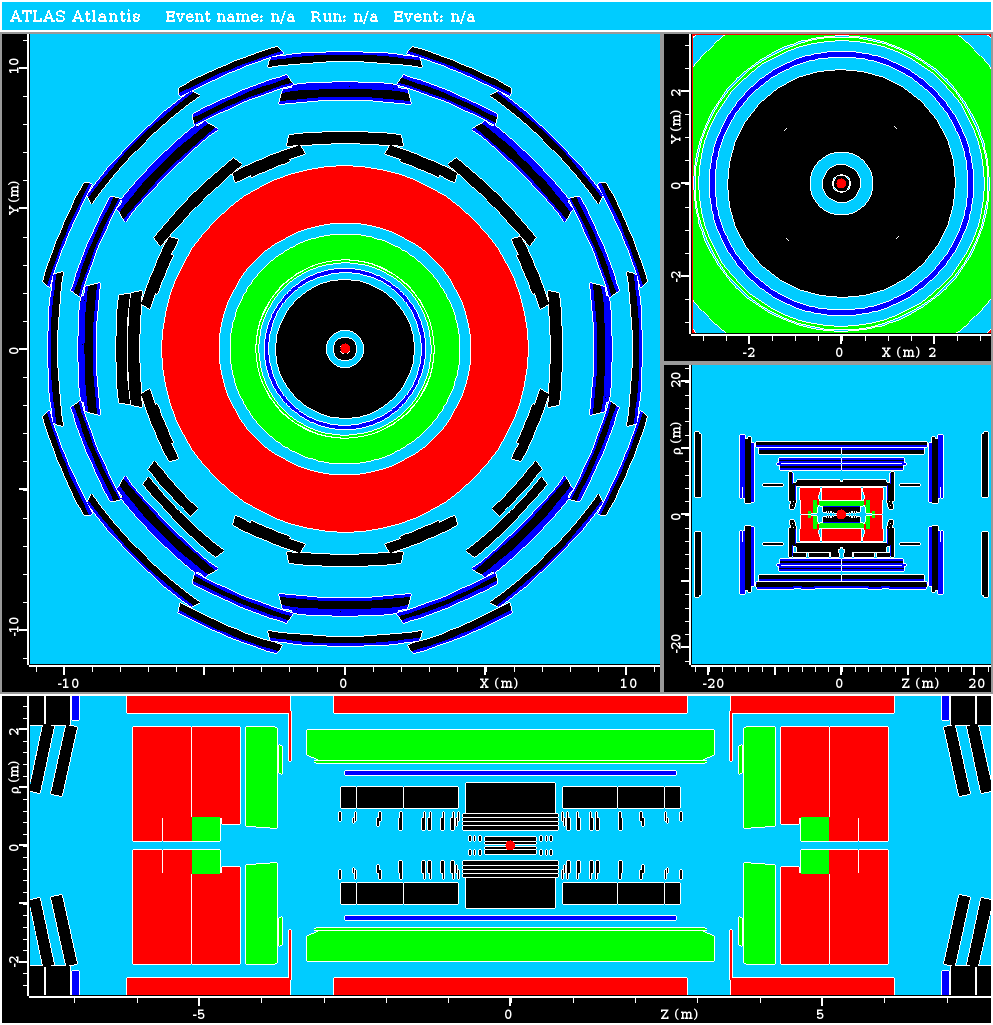
\includegraphics[width=\textwidth]{./data/atlantis/atlantis_empty.png}
	\caption{Hauptfenster des Atlantis-Programms in der Standardansicht}
	\label{fig:atlantis}
\end{figure}

\subsection{ROOT}
Zur Bearbeitung der Versuchsaufgaben 2 bis 4 wird das Datenanalyseprogramm ROOT verwendet.
ROOT wird über einen C++-Interpreter aus der Kommandozeile heraus gesteuert und bietet vielfältige Möglichkeiten zur Datenanalyse.
Die für den Versuch nötigen Daten und Funktionen werden als C++-Objekte vor Durchführung der Aufgaben in ROOT geladen.


\section{Graphische Darstellung von Teilchenreaktionen}

\subsection{Lerndatensätze}

Zu Beginn des Versuchs wurde der Umgang mit Atlantis geübt.
Hierzu wurden verschiedene Lerndatensätze betrachtet, die Ereignisse von Elektronen, Myonen, Photonen, $\tau$~-Leptonen und Jets enthalten.
Exemplarisch sollen für diese Teilchen im Folgenden einige Ereignisse vorgestellt werden, mit denen die Antwort des Detektors auf verschiedene Teilchenarten verstanden werden kann.

\clearpage
\subsubsection{Elektronen}
\begin{figure}[htbp]
	\centering
	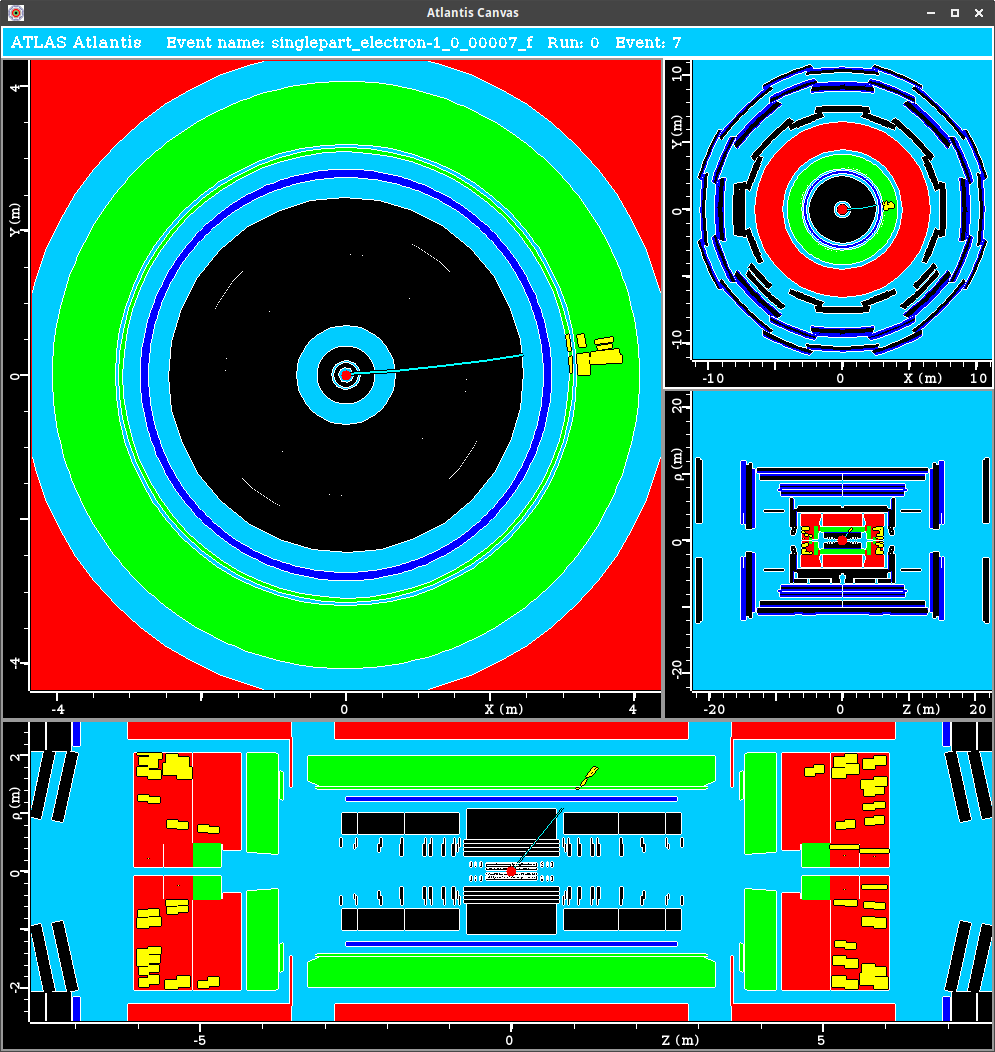
\includegraphics[width=1.0\textwidth]{./data/atlantis/singlepart_events_new/electron/curvature.png}
	\caption{Signatur eines einzelnen Elektrons im ATLAS-Detektor}
	\label{fig:electron-curvature}
\end{figure}
\vfill
\noindent
Im Lerndatensatz der Elektronen finden sich Ereignisse in denen einzelne Elektronen erzeugt wurden.
In Abbildung \ref{fig:electron-curvature} wurde ein typisches Ereignis mit einem einzelnen Elektron aufgetragen.
Die Signatur eines Elektrons ist gekennzeichnet durch eine Trajektorie im inneren Detektor, welche aufgrund der elektromagnetischen Interaktion des Elektrons mit dem Detektormaterial als Ladungseintrag in den Halbleiter- und Übergangsstrahlungsdetektoren rekonstruiert werden kann.
Das Magnetfeld im inneren Detektor, welches in Richtung der Strahlröhre zeigt, zwingt die Elektronen dort auf einen Kreisbogen und wird zur Rekonstruktion von Ladung und transversalem Impuls genutzt.
Im Fall von Abbildung \ref{fig:electron-curvature} kann an der Krümmung abgelesen werden, dass es sich um ein negativ geladenes Elektron handelt (das Magnetfeld zeigt in der $xy$-Ansicht aus der Bildebene).
Schließlich bildet das Elektron im elektromagnetischen Kalorimeter eine Kaskade aus Photonen und Elektron-Positron-Paaren aufgrund von Bremsstrahlungs- und Paarbildungsprozessen.
\vfill

\clearpage
\begin{figure}[htbp]
	\centering
	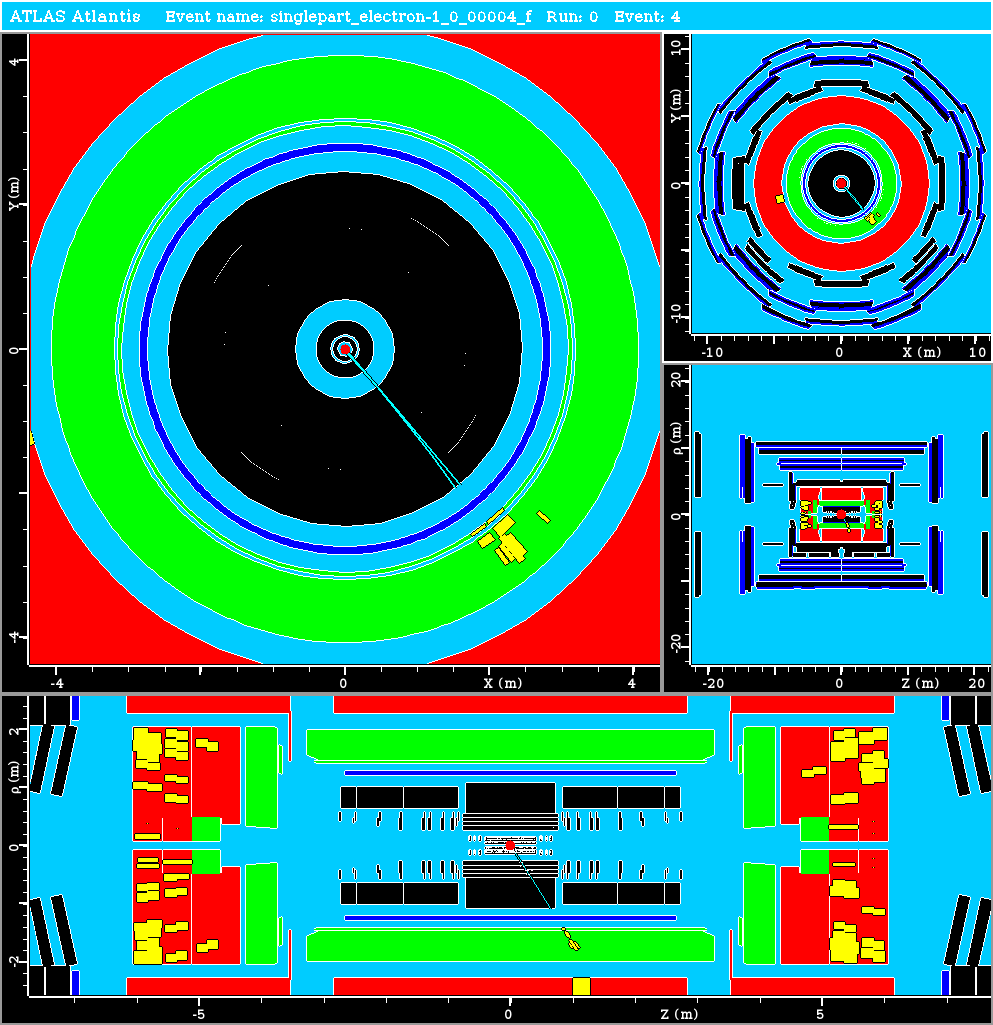
\includegraphics[width=1.0\textwidth]{./data/atlantis/singlepart_events_new/electron/twopart.png}
	\caption{Signatur eines Elektrons mit zusätzlichen geladenen Spuren im ATLAS-Detektor}
	\label{fig:electron-twopart}
\end{figure}
\vfill
\noindent
In Abbildung \ref{fig:electron-twopart} wurden zwei geladene Spuren im inneren Detektor rekonstruiert.
Da die zugrundeliegenden Ereignisse jedoch nur aus einem einzelnen Elektron bestehen, muss die zweite Spur durch das Ereignis-Elektron im Detektormaterial erzeugt worden sein.
Eine Möglichkeit dafür ist die Erzeugung eines hoch-energetischen Delta-Elektrons durch das Primärelektron.
Die Wahrscheinlichkeit für die Emission eines Delta-Elektrons in Vorwärtsrichtung ist jedoch sehr klein, daher könnte eine Alternative die Erzeugung eines Bremsstrahlphotons und die folgliche Paarbildung sein, in der das dritte Elektron nicht im Detektor rekonstruiert werden konnte.
\vfill

\clearpage
\subsubsection{Myonen}
\begin{figure}[htbp]
	\centering
	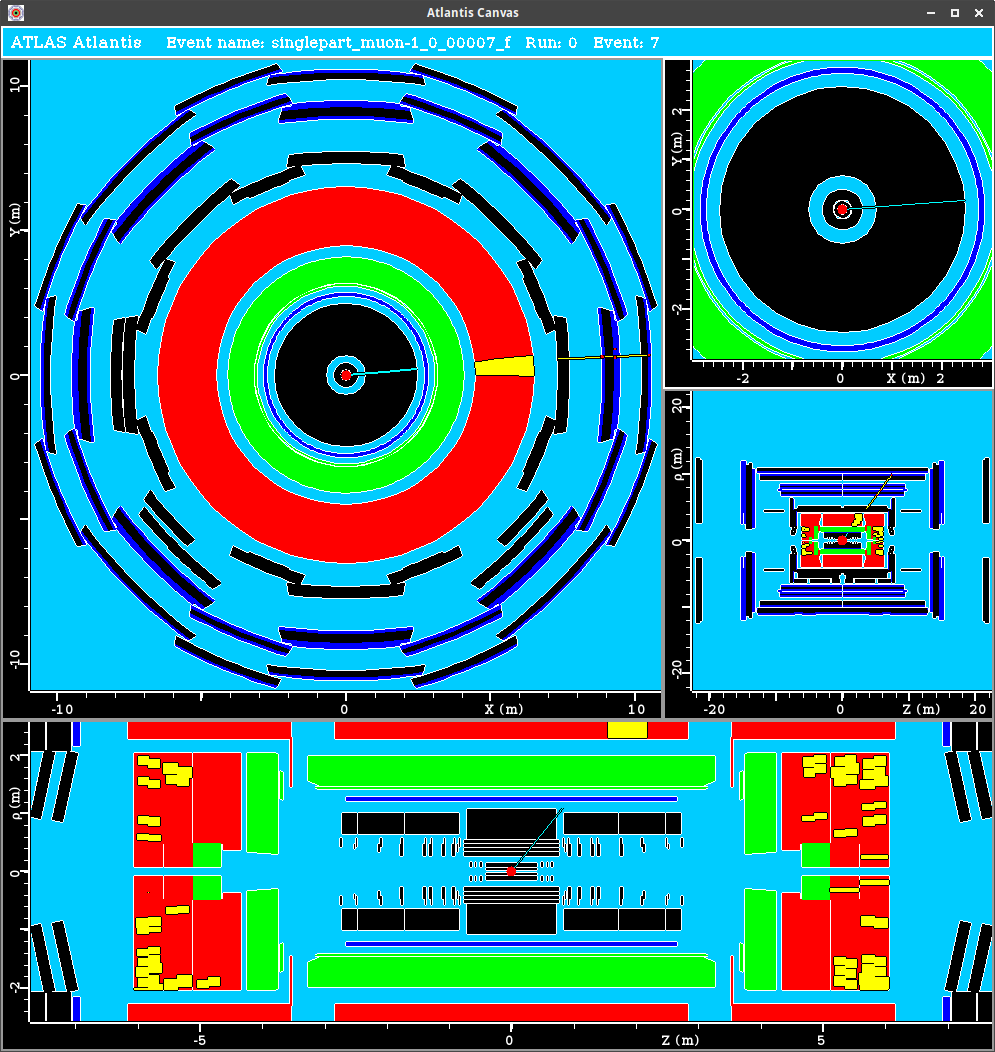
\includegraphics[width=1.0\textwidth]{./data/atlantis/singlepart_events_new/muon/single_track2.png}
	\caption{Signatur eines einzelnen Myons im ATLAS-Detektor}
	\label{fig:myon-singletrack}
\end{figure}
\vfill
\noindent
In Abbildung \ref{fig:myon-singletrack} ist die typische Detektorantwort auf ein Myon zu sehen.
Da es sich bei Myonen um geladene Teilchen handelt, hinterlassen diese eine Spur im inneren Detektor und passieren das dort anliegende Magnetfeld auf einer gekrümmten Bahn in der $xy$-Ebene.
Sie durchtreten die beiden Kalorimeter beinahe ungehindert und deponieren dabei nur eine geringe Energiemenge.
Im Myonsystem, das mit zahlreichen Detektorkammern und dem Magnetfeld eines toroidalen Spulensystems ausgestattet ist, können ebenfalls Spuren rekonstruiert werden.
Aufgrund des Magnetfeldes werden Myonen jedoch in der $\rho z$-Ebene gekrümmt, was eine zweite unabhängige Impulsmessung ermöglicht.
Da andere hadronische oder leptonische Teilchen im elektromagnetischen oder hadronischen Kalorimeter gestoppt werden und Neutrinos keine Spuren in den Detektorkammern des Myonsystems hinterlassen, ist diese Teilchensignatur auf ein Myon zurückzuführen. 
\vfill

\clearpage
\subsubsection{Photonen}
\begin{figure}[htbp]
	\centering
	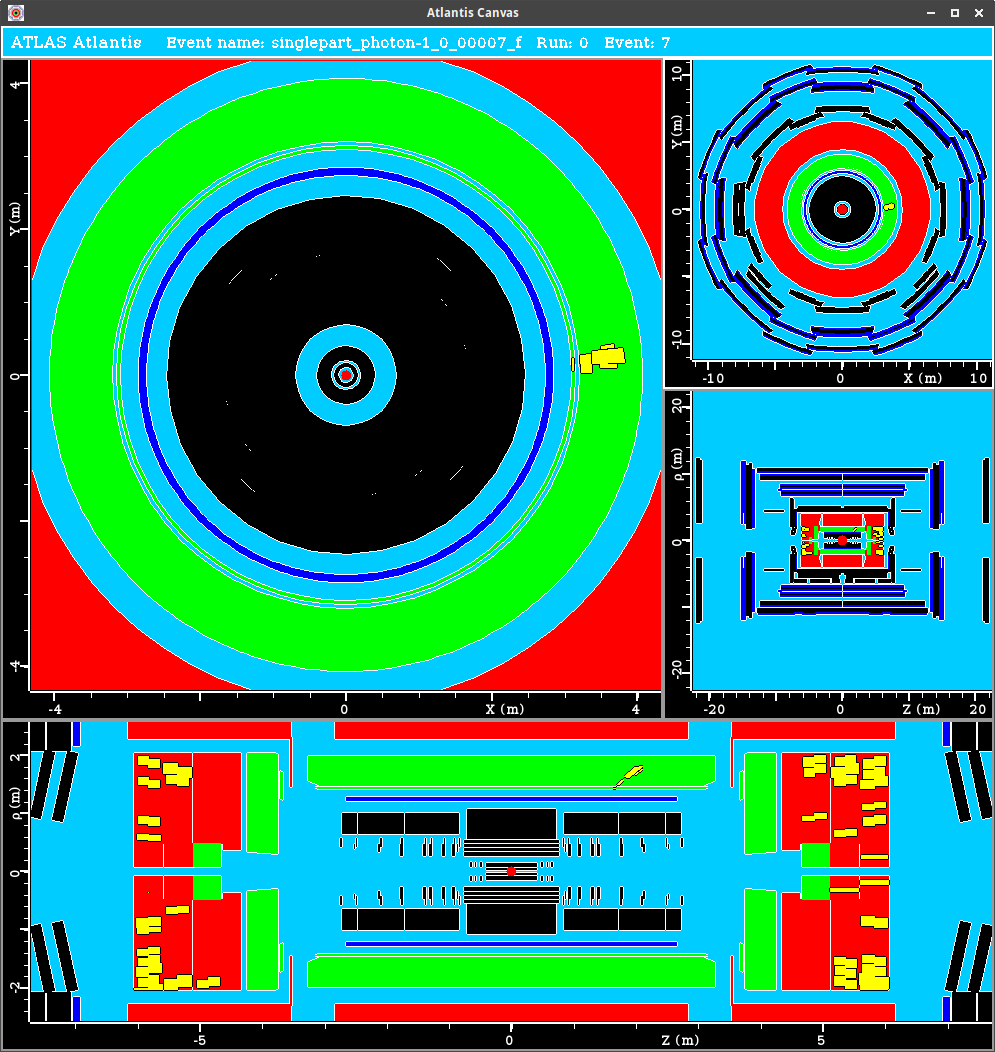
\includegraphics[width=1.0\textwidth]{./data/atlantis/singlepart_events_new/photons/single_photon_2.png}
	\caption{Signatur eines einzelnen Photons im ATLAS-Detektor}
	\label{fig:photon}
\end{figure}
\vfill
\noindent
Wie in Abbildung \ref{fig:photon} zu sehen, hinterlassen Photonen als ungeladene Teilchen keine rekonstruierbaren Spuren im inneren Detektor.
Da sie jedoch elektromagnetisch mit Materie interagieren können, formt sich im elektromagnetischen Kalorimeter ein Schauer aus Photonen und Elektron-Positron-Paaren (ähnlich zum Elektron).
In dieser Kaskade wird die gesamte Energie des Photons deponiert.
\vfill

\clearpage
\begin{figure}[htbp]
	\centering
	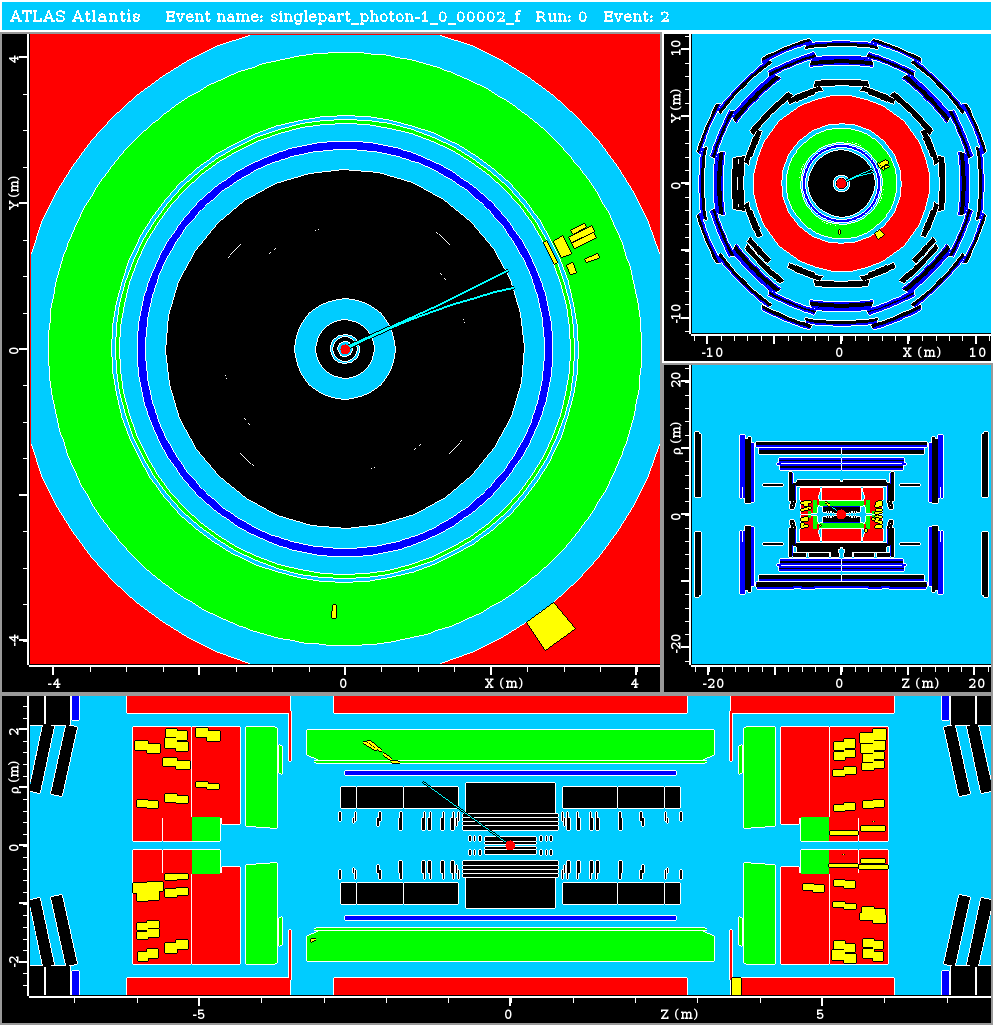
\includegraphics[width=1.0\textwidth]{./data/atlantis/singlepart_events_new/photons/conversion.png}
	\caption{Signatur eines $\mathrm{e}^- \mathrm{e}^+$-Paares aus dem Paarbildungsprozess eines einzelnen Photons im ATLAS-Detektor}
	\label{fig:photon-conversion}
\end{figure}
\vfill
\noindent
Im Ereignis in Abbildung \ref{fig:photon-conversion} entsteht ein Elektron-Positron-Paar durch Paarbildung des primären Photons im Detektormaterial.
Die Elektronen haben dabei entgegengesetzte Ladungen, sodass die Trajektorien im inneren Detektor in unterschiedliche Richtungen gekrümmt sind.
Darüber hinaus ist es möglich den gemeinsamen Vertex der Elektronen vom Interaktionsvertex zu unterscheiden.
Dies wurde in Abbildung \ref{fig:photon-vertex} mit der Vertexrekonstruktion von ATLANTIS dargestellt, sodass der sekundäre Vertex einen Abstand von etwa \SI{5}{\centi\meter} vom Interaktionsvertex hat.
\vfill
\begin{figure}[htbp]
	\centering
	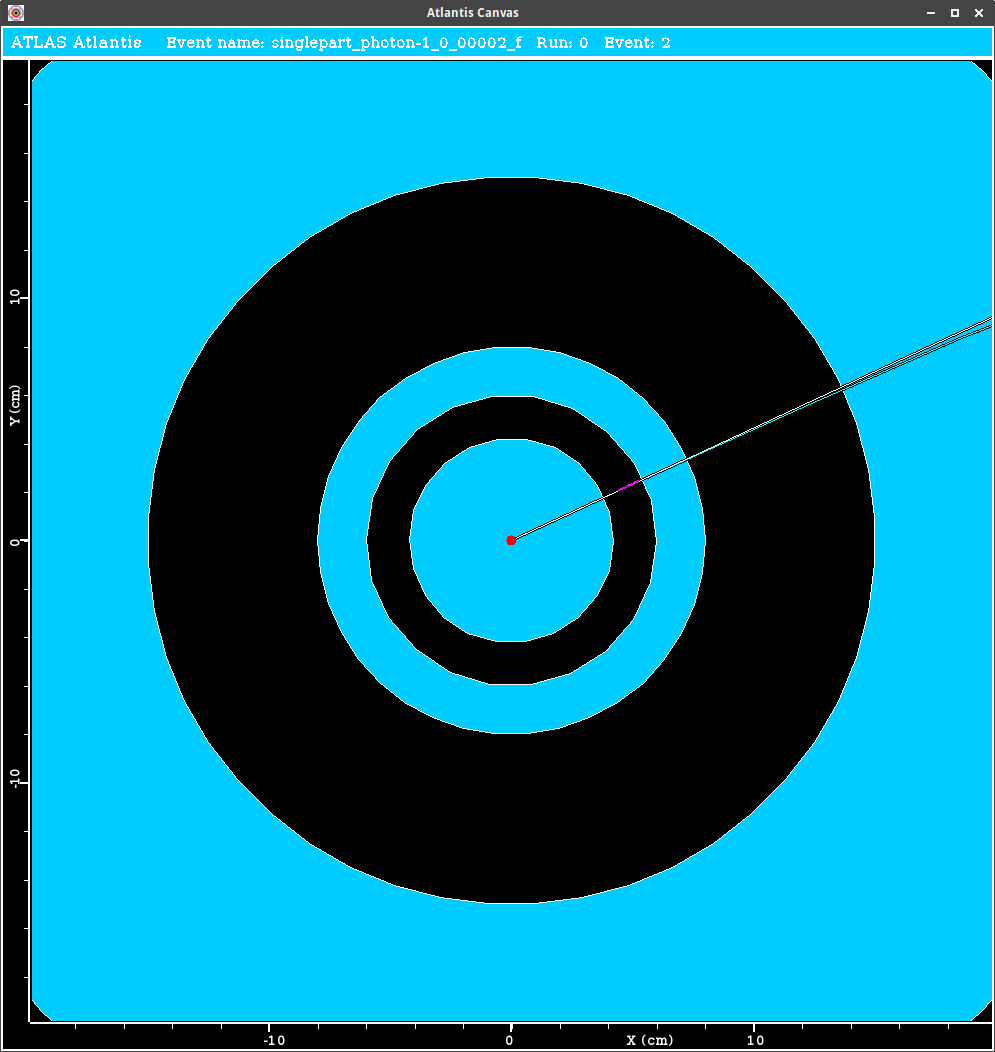
\includegraphics[width=1.0\textwidth]{./data/atlantis/singlepart_events_new/photons/conversion_vertex_no_fisheye.png}
	\caption{Von ATLANTIS rekonstruierter Vertex (magenta) des Elektron-Positron-Paars in einer Entfernung von etwa \SI{5}{\centi\meter} vom Interaktionsvertex (rot).}
	\label{fig:photon-vertex}
\end{figure}

\clearpage
\subsubsection{$\tau$-Leptonen}
\begin{figure}[htbp]
	\centering
	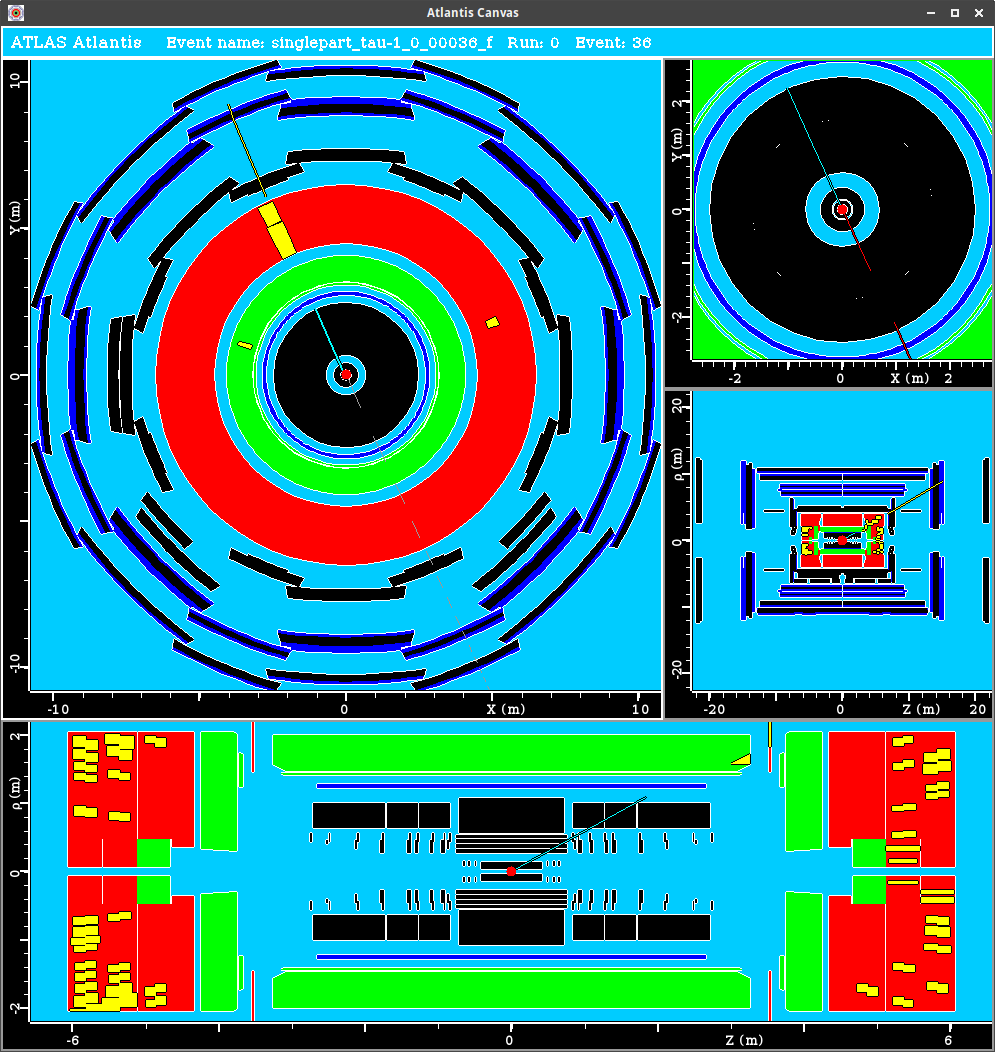
\includegraphics[width=1.0\textwidth]{./data/atlantis/singlepart_events_new/tau/muon.png}
	\caption{Signatur des leptonischen Zerfalls eines $\tau^+$-Leptons im ATLAS-Detektor.}
	\label{fig:tau-muon}
\end{figure}
\vfill
\noindent
Das Ereignis in Abbildung \ref{fig:tau-muon} des $\tau$-Lerndatensatzes zeigt den Zerfall
\begin{align*}
	\tau^+ \rightarrow \mu^+ + \nu_\mu + \bar{\nu}_\tau \, \text{.}
\end{align*}
Aufgrund der kurzen Lebensdauer zerfällt das $\tau$-Lepton nach sehr kurzer Flugstrecke $c \tau = \SI{87}{\micro\meter}$ \cite{pdg}, weshalb lediglich das Myon im Detektor rekonstruiert werden kann.
Aufgrund der Leptonen-Universalität ist auch ein Zerfall in Elektron und zugehöriges Neutrino  mit ungefähr dem gleichen Verzweigungsverhältnis (abgesehen vom Phasenraumunterschied) möglich.
Ein solcher Zerfall würde lediglich eine geladene Spur und einen Schauer im elektromagnetischen Kalorimeter verursachen und nicht wie bei dem hier betrachteten Ereignis im Myonsystem registriert werden.

In beiden Fällen entstehen zusätzlich zu dem geladenen Lepton auch ein $\tau$-Neutrino und das jeweilige Neutrino des Elektrons bzw.\ Myons.
Diese können nicht detektiert werden, die fehlende transversale Energie (in den beiden oberen Ansichten der Abbildung \ref{fig:tau-muon} rot bzw.\ grau gestrichelt) ist jedoch ein Indiz für ihre Existenz.
\vfill

\clearpage
\begin{figure}[htbp]
	\centering
	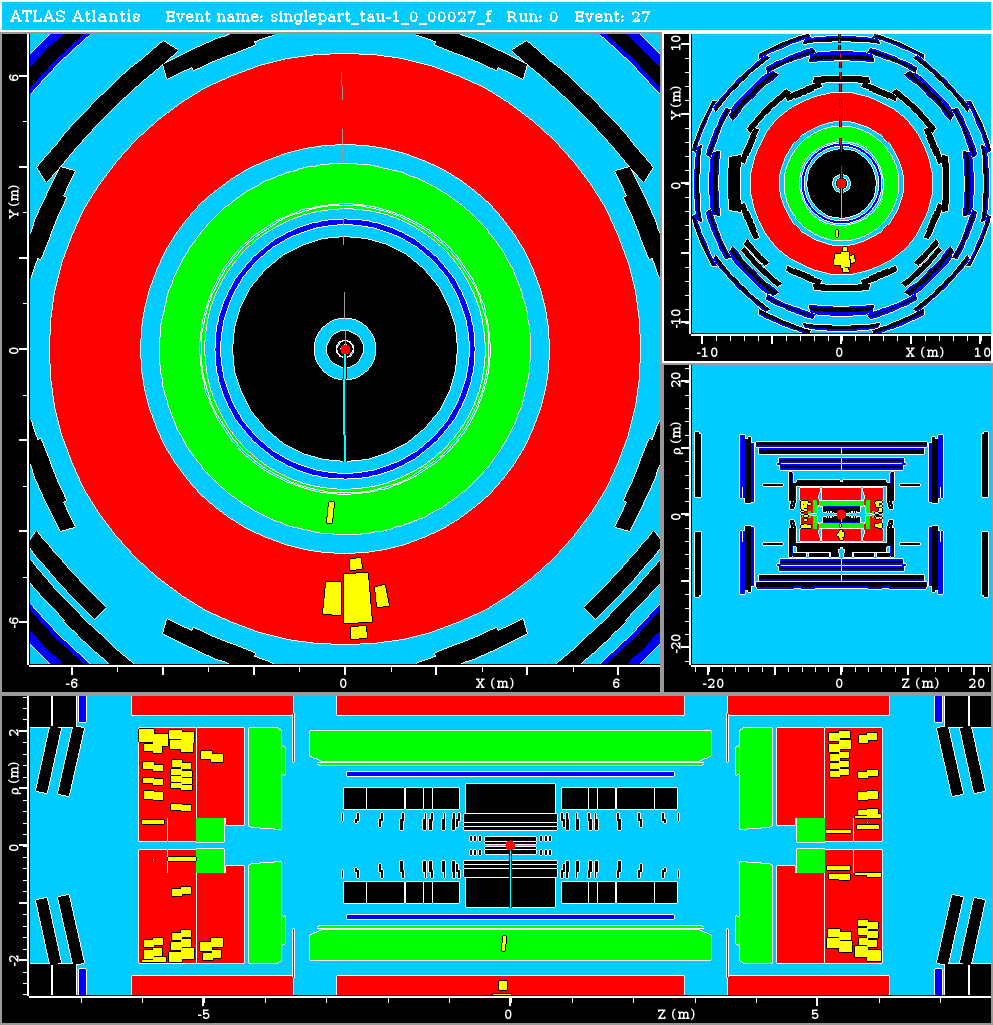
\includegraphics[width=1.0\textwidth]{./data/atlantis/singlepart_events_new/tau/single_pion.png}
	\caption{Signatur eines hadronischen $\tau$-Zerfalls im ATLAS-Detektor}
	\label{fig:tau-pion}
\end{figure}
\vfill
\noindent
Ein Beispiel für einen hadronischen $\tau$-Zerfall liefert Abbildung \ref{fig:tau-pion}.
In diesem Fall ist eine geladene Spur im inneren Detektor sichtbar, sodass ein Zerfall mit einem geladenen Pion und einem $\tau$-Neutrino im Endzustand stattgefunden haben muss.
Weiterhin können noch bis zu drei neutrale Pionen auftreten, welche nicht im inneren Detektor sichtbar sind.
Aufgrund der Lokalisierung der Energie im hadronischen Kalorimeter in einem kleinen Raumbereich ist ein Zerfall in ein einzelnes geladenes Pion zu vermuten.
Es ist ebenfalls die fehlende transversale Energie aufgrund des $\tau$-Neutrinos zu beobachten, welche im Gegensatz zum leptonischen Zerfall nun ein Maß für den transversalen Impuls des Neutrinos darstellt, da nur ein Neutrino bei diesem Ereignis auftritt.
\vfill

\clearpage
\subsubsection{Zwei-Jet}
\begin{figure}[htbp]
	\centering
	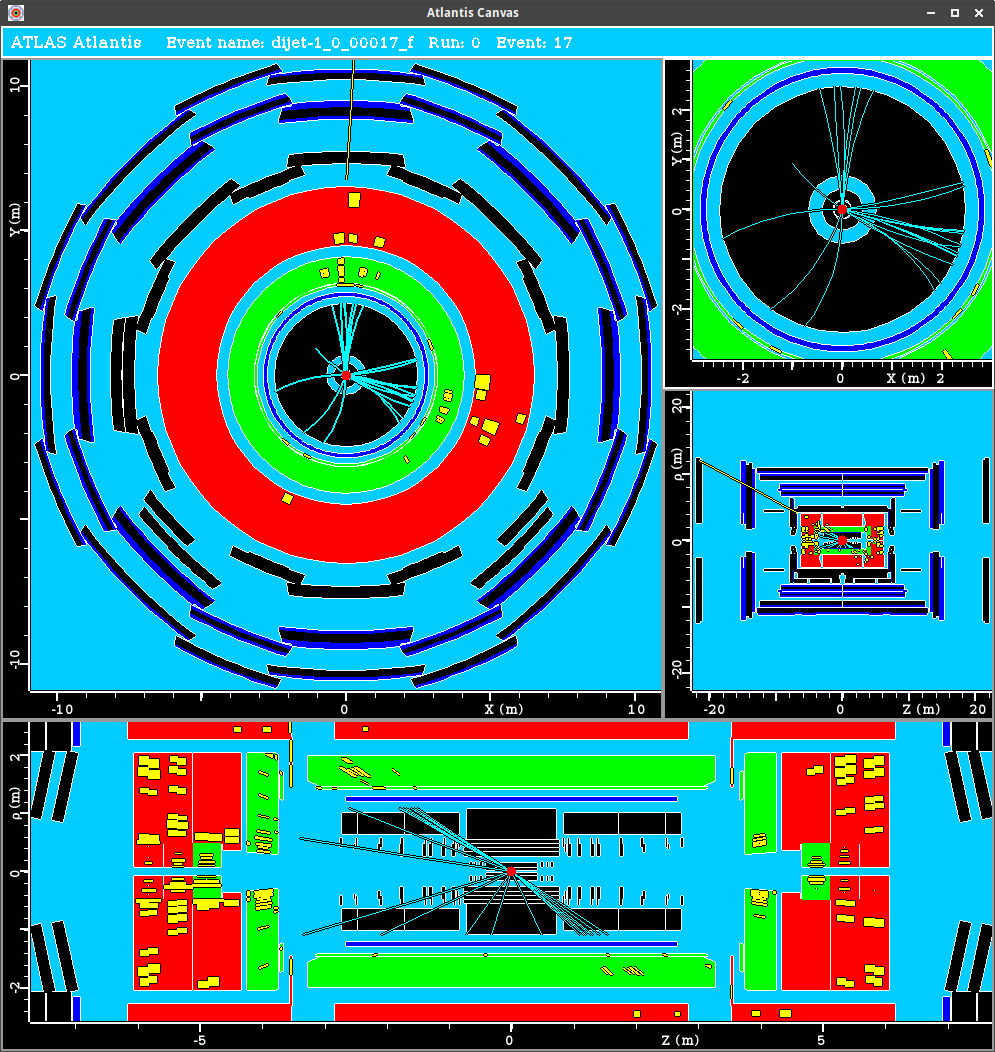
\includegraphics[width=1.0\textwidth]{./data/atlantis/singlepart_events_new/jets/muon.png}
	\caption{Signatur eines Zwei-Jet Ereignisses im ATLAS-Detektor}
	\label{fig:jets-muon}
\end{figure}
\vfill
\noindent
In dem in Abbildung \ref{fig:jets-muon} zugrundeliegenden Ereignis entstehen zwei Quarks oder Gluonen, welche folglich aufgrund des \textit{Confinements} zwischen farb-geladenen Teilchen in Mesonen und Baryonen hadronisieren.
Die so entstehenden geladenen Hadronen bilden im inneren Detektor eine Ansammlung vieler Spuren in einem engen Konus.
Ein solcher \textit{Jet} enthält sowohl geladene als auch ungeladene Pionen.
Die geladenen Pionen haben eine Zerfallslänge in der Ordnung von $c \tau = \SI{7.8}{\meter}$~\cite{pdg} und können dadurch direkt in den hadronischen Kalorimetern beobachtet werden.
Im Gegensatz dazu zerfallen die ungeladenen Pionen schnell in zwei Photonen ($c \tau = \SI{25.5}{\nano\meter}$~\cite{pdg}) und führen somit ebenfalls zu signifikanten Einträgen in den elektromagnetischen Kalorimetern.

Das Myon, welches im oberen Jet in Abbildung \ref{fig:jets-muon} zu erkennen ist, ist ein Indikator dafür, dass das hadronisierende Quark-Paar ein $b\bar{b}$-Paar gewesen ist, da der Zerfall des im Jet entstandenen B-Mesons zu einem geladenen Lepton im Endzustand führen kann.
\vfill

\subsection{Energieverlust von Myonen in den Kalorimetern des ATLAS-Detektors}
Im Folgenden soll anhand der ersten 20 Myonen-Ereignisse aus den Lerndatensätzen der mittlere Energieverlust der Myonen in den Kalorimetern bestimmt werden. 

\subsubsection{Bestimmung des Myonenimpulses mit Atlantis}
\label{sssec:myon_momenta}
Der ATLAS-Detektor besitzt mit dem Magnetfeld des Solenoids im inneren Detektor und dem des toroidalen Spulensystems im Myonensystem zwei unabhängige Methoden um den Myonenimpuls zu bestimmen.
Bei den betrachteten Ereignissen können mithilfe der Ereignisanzeige Atlantis die Parameter (Impuls~$p$, transversaler Impuls~$p_\mathrm{T}$, Pseudorapidität~$\eta$, \dots) der Myonen jeweils im inneren Detektor und im Myonensystem abgefragt werden.

Um den Energieverlust der Myonen im Kalorimeter zu bestimmen, ist es nötig den Impuls~$p$ ebendieser zu bestimmen.
Da Atlantis auf diesen Parameter jedoch keinen Fehler angibt, wurde stattdessen der transversale Impuls~$p_\mathrm{T}$ und die Pseudorapidität~$\eta$ genutzt, um die Fehlerfortpflanzung per Hand durchzuführen.
Nach der Definition in Gleichung \eqref{eq:pseudorapidity} und $p = p_\mathrm{T} / \sin\vartheta$ kann der Impuls gemäß
\begin{align*}
	p = p_\mathrm{T} \cosh(\eta)
\end{align*}
berechnet werden.
Da der relative Fehler der Pseudorapidität gemäß Atlantis in der Größenordnung $10^{-3}$ liegt, soll dieser im Folgenden vernachlässigt werden.
Dann folgt aus \textsc{Gauß}scher Fehlerfortpflanzung für den Fehler des Impulses
\begin{align*}
	\sigma_p = | \cosh(\eta) \cdot \sigma_{p_\mathrm{T}} | \, \text{.}
\end{align*}
Die Messdaten sowie die Berechnung des Impulses~$p$ der Myonen im inneren Detektor und des Impulses~$p^\prime$ im Myon-Detektor wurde in Tabelle \ref{tab:muon_momenta} zusammengetragen.

Bei dem 10.\ Ereignis musste festgestellt werden, dass keine Trajektorie im Myon-Detektor rekonstruiert werden konnte.
Der Vergleich mit dem Pfad des Myons im inneren Detektor legt dabei nahe, dass dieses durch einen nicht-sensitiven Bereich des Detektors zwischen Barrel und Endkappe entkommen konnte.
Daher wurde zusätzlich das 21.\ Ereignis vermessen.


\begin{sidewaystable}
	\centering
	\begin{tabular}{rSSSSSSSSSS}
\toprule
{Ereignis} & {$p_T$ / \si{\GeV}} & {$\sigma_{p_T}$ / \si{\GeV}} & {$\eta$} & {$p$ / \si{\GeV}} & {$\sigma_p$ / \si{\GeV}} & {$p_T^\prime$ / \si{\GeV}} & {$\sigma_{p_T^\prime}$ / \si{\GeV}} & {$\eta^\prime$} & {$p^\prime$ / \si{\GeV}} & {$\sigma_{p^\prime}$ / \si{\GeV}} \\
\midrule
         1 &               -38.4 &                          1.0 &     1.44 &             -85.3 &                      2.3 &                      -24.1 &                                 2.6 &            1.45 &                    -53.9 &                               5.8 \\
         2 &                33.2 &                          0.8 &    -0.77 &              43.4 &                      1.0 &                       33.4 &                                 1.7 &           -0.77 &                     43.8 &                               2.2 \\
         3 &               -41.9 &                          3.6 &    -2.44 &            -241.4 &                     21.0 &                      -41.0 &                                 0.7 &           -2.44 &                   -236.9 &                               3.8 \\
         4 &                42.0 &                          0.8 &     0.57 &              48.9 &                      1.0 &                       38.1 &                                 1.3 &            0.58 &                     44.8 &                               1.6 \\
         5 &               -53.7 &                          2.1 &    -1.81 &            -168.2 &                      6.4 &                      -61.2 &                                 4.4 &           -1.73 &                   -177.6 &                              12.8 \\
         6 &                44.6 &                          1.4 &     1.62 &             117.3 &                      3.6 &                       36.6 &                                 3.1 &            1.62 &                     96.5 &                               8.3 \\
         7 &               -57.3 &                          1.7 &     0.70 &             -71.9 &                      2.1 &                      -51.8 &                                 1.1 &            0.70 &                    -65.0 &                               1.3 \\
         8 &                64.5 &                          2.7 &     1.80 &             200.0 &                      8.3 &                       64.9 &                                 2.8 &            1.79 &                    199.3 &                               8.7 \\
         9 &               -55.5 &                          1.1 &    -0.29 &             -57.8 &                      1.2 &                      -48.0 &                                 0.9 &           -0.27 &                    -49.7 &                               1.0 \\
        10 &                39.9 &                          1.0 &     1.18 &              71.1 &                      1.7 &                            &                                     &                 &                          &                                   \\
        11 &               -37.8 &                          1.2 &    -1.64 &            -100.7 &                      3.2 &                      -35.1 &                                 0.7 &           -1.65 &                    -94.3 &                               1.8 \\
        12 &                37.6 &                          0.7 &     0.19 &              38.3 &                      0.7 &                       33.9 &                                 1.2 &            0.19 &                     34.5 &                               1.2 \\
        13 &               -59.9 &                          1.8 &     1.16 &            -105.2 &                      3.1 &                      -62.1 &                                 4.2 &            1.16 &                   -108.7 &                               7.3 \\
        14 &                47.5 &                          3.3 &     2.29 &             236.1 &                     16.5 &                       53.0 &                                 1.2 &            2.29 &                    263.5 &                               5.9 \\
        15 &               -43.9 &                          1.5 &    -1.76 &            -131.7 &                      4.4 &                      -42.0 &                                 2.1 &           -1.76 &                   -125.5 &                               6.3 \\
        16 &                45.7 &                          1.8 &    -1.87 &             152.2 &                      6.1 &                       47.3 &                                 2.2 &           -1.88 &                    157.7 &                               7.2 \\
        17 &               -32.6 &                          0.5 &     0.40 &             -35.2 &                      0.6 &                      -29.8 &                                 0.5 &            0.40 &                    -32.2 &                               0.6 \\
        18 &                52.8 &                          1.1 &     0.23 &              54.2 &                      1.1 &                       48.7 &                                 2.3 &            0.23 &                     50.0 &                               2.3 \\
        19 &               -64.5 &                          2.5 &     0.77 &             -84.7 &                      3.3 &                      -52.2 &                                 1.0 &            0.76 &                    -68.1 &                               1.4 \\
        20 &                47.6 &                          1.3 &     1.42 &             104.2 &                      2.9 &                       49.5 &                                 3.2 &            1.42 &                    108.0 &                               7.0 \\
        21 &               -35.5 &                          2.3 &    -2.33 &            -184.1 &                     11.8 &                      -33.2 &                                 0.8 &           -2.32 &                   -170.8 &                               4.0 \\
\bottomrule
\end{tabular}

	\caption{Bestimmung des Impulses des Myons im inneren Detektor (ungestrichene Größen) und im Myonensystem (gestrichene Größen) mithilfe der gemessenen Pseudorapidität~$\eta$ und des transversalen Impulses~$p_\mathrm{T}$.
		Für Ereignis 10 konnte kein äußeres Myon rekonstruiert werden (für weitere Erklärung siehe Abschnitt \ref{sssec:myon_momenta}) stattdessen wurde noch das 21.\ Ereignis in die Analyse einbezogen.
		Das Vorzeichen von ~$p_\mathrm{T}$ dient der Unterscheidung positiv und negativ geladener Teilchen.}
	\label{tab:muon_momenta}
\end{sidewaystable}

\subsubsection{Bestimmung von Impuls- und Energieverlust der Myonen im Kalorimeter}
Nachfolgend soll der Impuls- bzw.\ Energieverlust der vermessenen Myonen im Kalorimeter berechnet werden.
Zunächst betrachte man, dass der Myonenimpuls~$p^{(\prime)}$ in der Größenordnung von einigen \SI{10}{\GeV} liegt.
Im Vergleich dazu beträgt die Masse der Myonen
\begin{align*}
	m_\mu \approx \SI{105.658}{\MeV} \, \cite{pdg} \text{,}
\end{align*}
weshalb $p \gg m_\mu$ ist und dadurch in guter Approximation $p^{(\prime)} = E^{(\prime)}$ angenommen werden kann.

Anschließend kann der Impuls- und Energieverlust aus der Differenz von Myon-Impuls im inneren Detektor~$p$ und Myon-Impuls im Myon-Detektor~$p^\prime$ berechnet werden:
\begin{align}
	\Delta E \approx \Delta p = p - p^\prime
	\label{eq:p_diff}
\end{align}
und der Fehler nach \textsc{Gauß}scher Fehlerfortpflanzung
\begin{align*}
	\sigma_{\Delta E} = \sqrt{\sigma_p^2 + \sigma_{p^\prime}^2} \, \text{.}
\end{align*}
Die somit berechneten Energieverluste wurden in Tabelle \ref{tab:energy_loss_muons} aufgetragen.
Anzumerken ist, dass für die Auswertung von Gleichung \eqref{eq:p_diff} das Ladungsvorzeichen, welches von Atlantis auf alle Impulse angegeben wird, verworfen wurde.

\begin{table}[h]
	\centering
	\begin{subtable}{.5\textwidth}
		\centering		
		\begin{tabular}{rSS}
\toprule
{Ereignis} & {$\Delta E$ / \si{\GeV}} & {$\sigma_{\Delta E}$ / \si{\GeV}} \\
\midrule
         1 &                     31.4 &                               6.2 \\
         2 &                     -0.4 &                               2.4 \\
         3 &                      4.5 &                              21.3 \\
         4 &                      4.1 &                               1.8 \\
         5 &                     -9.4 &                              14.3 \\
         6 &                     20.8 &                               9.1 \\
         7 &                      7.0 &                               2.5 \\
         8 &                      0.7 &                              12.1 \\
         9 &                      8.1 &                               1.5 \\
        11 &                      6.4 &                               3.6 \\
\bottomrule
\end{tabular}
	
	\end{subtable}%
	\begin{subtable}{.5\textwidth}
		\centering
		\begin{tabular}{rSS}
\toprule
{Ereignis} & {$\Delta E$ / \si{\GeV}} & {$\sigma_{\Delta E}$ / \si{\GeV}} \\
\midrule
        12 &                      3.8 &                               1.4 \\
        13 &                     -3.5 &                               8.0 \\
        14 &                    -27.4 &                              17.5 \\
        15 &                      6.2 &                               7.7 \\
        16 &                     -5.5 &                               9.5 \\
        17 &                      3.1 &                               0.8 \\
        18 &                      4.2 &                               2.6 \\
        19 &                     16.7 &                               3.6 \\
        20 &                     -3.8 &                               7.6 \\
        21 &                     13.3 &                              12.5 \\
\bottomrule
\end{tabular}

	\end{subtable}
	\caption{Energieverlust~$\Delta E$ der Myonen im Kalorimeter des ATLAS-Detektors. Negative $\Delta E$ entsprechen einer Energiezunahme.}
	\label{tab:energy_loss_muons}
\end{table}

\subsubsection{Energieverlust und dessen Abhängigkeiten}
Betrachtet man den Energieverlust der Myonen in Tabelle \ref{tab:energy_loss_muons}, so stellt man fest, dass bei einigen Ereignissen ein negativer Energieverlust gemessen wurde.
Dies entspricht einem Energiegewinn der Myonen in den Kalorimetern und ist unphysikalisch.
Betrachtet man jedoch den Fehler dieser Größen, sind die meisten dieser unphysikalischen Myonen noch mit positiven Energieverlusten kompatibel.

Im Folgenden sollen die Abhängigkeiten des Energieverlustes von den kinematischen Variablen der Myonen untersucht werden.
Zunächst würde man erwarten, dass eine Abhängigkeit von der Pseudorapidität~$\eta$ existiert, da die Weglängen der Myonen durch die Kalorimeter bei unterschiedlichen Polarwinkeln~$\theta$ verschieden sind und somit im Mittel unterschiedliche Energieverluste zu erwarten sind.
Explizit würde man eine Zunahme des Energieverlustes mit steigender Pseudorapidität erwarten.
In Abbildung \ref{fig:muon_eloss_eta} wurde der Energieverlust gegen den Betrag der Pseudorapidität aufgetragen, welche zeigt, dass keine starke Abhängigkeit festgestellt werden kann.
Die Gründe dafür folgen nach dem nächsten Paragraphen.

Darüber hinaus ist eine starke Abhängigkeit von der Energie der Myonen zu erwarten, wenn diese größer ist als die kritische Energie\footnote{Myonenenergie mit gleichem Beitrag zum mittleren Energieverlust durch Ionisation und Bremsstrahlung: $\langle \frac{\mathrm{d}E}{\mathrm{d}x} \rangle_\mathrm{Ion.}(E_{\mu\mathrm{c}}) = \langle \frac{\mathrm{d}E}{\mathrm{d}x} \rangle_\mathrm{Brems.}(E_{\mu\mathrm{c}})$}~$E_{\mu\mathrm{c}}$ der Myonen im Kalorimetermaterial.
Da diese jedoch in der Größenordnung von mehreren \SI{100}{\GeV} \cite{pdg} liegt und der größte vermessene Impuls lediglich \SI{200}{\GeV} beträgt, sollte diese Abhängigkeit nicht in Erscheinung treten.
Zum Vergleich wurde auch hier die Abhängigkeit in Abbildung \ref{fig:muon_eloss_momentum} dargestellt.
\begin{figure}[hp]
	\begin{subfigure}{1.0\textwidth}
		\centering
		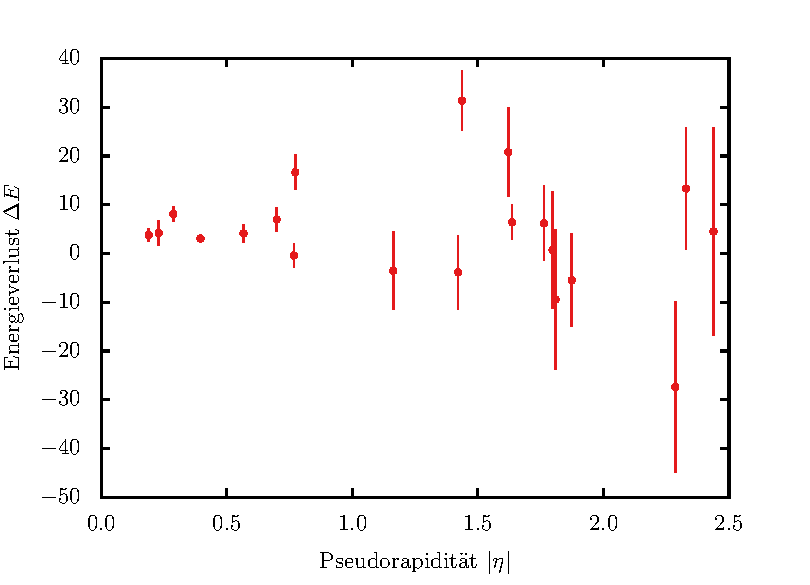
\includegraphics{./figures/muon_energy_loss/eta.pdf}
		\subcaption{}
		\label{fig:muon_eloss_eta}
	\end{subfigure}
	\begin{subfigure}{1.0\textwidth}
			\centering
			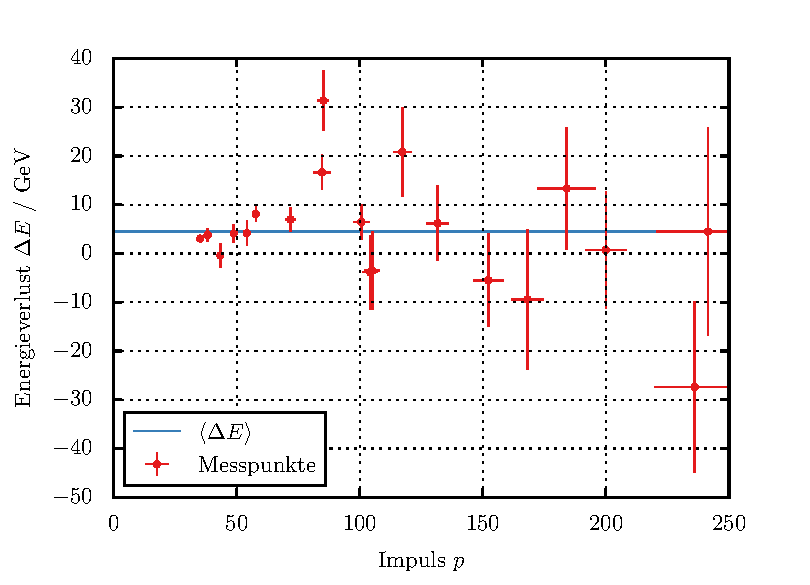
\includegraphics{./figures/muon_energy_loss/momentum.pdf}
			\subcaption{}
			\label{fig:muon_eloss_momentum}
	\end{subfigure}
	\caption{Abhängigkeiten des Energieverlustes der Myonen in den Kalorimetern des ATLAS-Detektors von der Pseudorapidität~$\eta$ des Myons und dessen Impuls~$p$. Ebenfalls aufgetragen ist eine Anpassung des mittleren Energieverlustes~$\langle \Delta E \rangle$.}
	\label{fig:muon_eloss}
\end{figure}

In beiden Fällen ist in Anbetracht der Fehler keine signifikante Abhängigkeit zu erkennen.
Im Wesentlichen liegt dies daran, dass der Energieverlust von Teilchen in Materie ein statistischer Prozess ist und man lediglich eine Distribution für diesen angeben kann (Laundau-Distribution).
Um eine bessere Bestimmung der Abhängigkeiten durchzuführen, sollten mehrere Energieverluste bei der gleichen zugrundeliegenden Größe (z.B.\ $\eta$, $p$, \dots) gemessen werden, um aus diesen einen Mittelwert zu bilden.

Schließlich soll der mittlere Energieverlust~$\Delta E$ der Myonen in den Kalorimetern berechnet werden.
Da keine signifikanten Abhängigkeiten aus den oben genannten Gründen festgestellt werden konnte, wird der mittlere Energieverlust durch eine $\chi^2$-Anpassung einer konstanten Funktion an die Daten durchgeführt.
Dadurch erhält man
\begin{align*}
	\langle \Delta E \rangle = \SI{4.46 +- 0.92}{\GeV}
\end{align*}
mit einem reduzierten $\chi$-Quadrat $\chi_\mathrm{red.}^2 = \num{3.11}$; das Ergebnis wurde ebenfalls in den Abbildungen \ref{fig:muon_eloss} aufgetragen.
Das reduzierte $\chi$-Quadrat spricht für keine gute Übereinstimmung der Fithypothese mit den gemessenen Daten, was jedoch nicht verwunderlich ist, da wie bereits erwähnt, der Energieverlust der Myonen einer statistischen Distribution folgt.

\subsection{Invariante Elektron-Positron-Masse im Prozess~$\mathrm{Z}^0 \rightarrow \mathrm{e}^+ + \mathrm{e}^-$}
Im Folgenden sollen aus einem Datensatz von Zerfällen~$\mathrm{Z}^0 \rightarrow \mathrm{e}^+ + \mathrm{e}^-$ drei Ereignisse gewählt werden und aus den rekonstruierten Elektronen die invariante Elektron-Positron-Masse bestimmt werden.
Bei der Auswahl der Ereignisse wurden die folgenden Bedingung gestellt:
\begin{itemize}
	\item zwei Elektronen mit hohem transversalen Impuls~$p_\mathrm{T}$
	\item eindeutig zuzuordnende Schauer im elektromagnetischen Kalorimeter
	\item entgegengesetzt Ladung beider Elektronen
\end{itemize}
Gemäß dieser Bedingungen wurden die Ereignisse 23, 33 und 37 des Datensatzes für die Auswertung ausgewählt.
Um die invariante Masse dieses Elektronen-Paares zu bestimmen, ist es notwendig den vektoriellen Impuls $\vec{p}$ beider Teilchen zu bestimmen.
Dazu wurde mithilfe von Atlantis der transversale Impuls~$p_\mathrm{T}$, die Pseudorapidität~$\eta$ und der Azimuthalwinkel~$\phi$ der rekonstruierten Elektronen bestimmt.
Die invariante Masse~$m_\mathrm{inv}$ kann dann gemäß
\begin{align*}
	m_\mathrm{inv}=\sqrt{(\mathbf{p}_{\mathrm{e}^-}+\mathbf{p}_{\mathrm{e}^+})^2}
\end{align*}
aus den beiden Vierervektoren von Elektron und Positron,~$\mathbf{p}_{\mathrm{e}^-}$ bzw.~$\mathbf{p}_{\mathrm{e}^+}$ berechnet werden.
Man erhält somit als Ausdruck für die invariante Masse
\begin{align}
	m_\mathrm{inv}&=\sqrt{2 m^2_{\mathrm{e}} + 2 ( E_{\mathrm{e}^-} E_{\mathrm{e}^+} - \vec{p}_{\mathrm{e}^-}\vec{p}_{\mathrm{e}^+} )} \nonumber \\
	&=\sqrt{ 2m^2_{\mathrm{e}} + 2 (E_{\mathrm{e}^-} E_{\mathrm{e}^+} - |\vec{p}_{\mathrm{e}^-}||\vec{p}_{\mathrm{e}^+}|\cos\theta)}\,\text{,}
	\label{eq:inv_mass}
\end{align}
wobei $\theta$ der Winkel zwischen den Impulsen beider Teilchen ist.
Da nur der Betrag des Impulses eines Teilchens gemessen werden kann, werden die Winkelinformationen~$\phi$ und~$\eta$ benötigt, um auf~$\theta$ zu schließen.
Dazu wird zunächst der Polarwinkel~$\vartheta$ im Laborsystem durch
\begin{align*}
	\vartheta = 2 \arctan\left( \mathrm{e}^{-\eta} \right)
\end{align*}
berechnet (folgt aus Gleichung \ref{eq:pseudorapidity}).
Anschließend können mit den Winkeln~$\phi$ und $\vartheta$ des sphärischen Koordinatensystems Einheitsvektoren in die Richtung der Elektronenimpulse durch
\begin{align*}
	\hat{p}_x = \sin\vartheta \cos\phi \qquad
	\hat{p}_y = \sin\vartheta \sin\phi \qquad
	\hat{p}_z = \cos\vartheta
\end{align*}
konstruiert werden.
Der Kosinus des Winkels zwischen dem Elektron- und Positronimpuls folgt dann aus dem Skalarprodukt
\begin{align*}
	\cos \theta = \hat{\vec{p}}_{\mathrm{e}^-} \cdot \hat{\vec{p}}_{\mathrm{e}^+}
\end{align*}
Bei der Berechnung dieses Werts kann aufgrund der kleinen Fehler in $\eta$ und $\phi$ der Fehler in~$\cos\theta$ vernachlässigt werden.
Außerdem muss noch der Betrag des Impulses~$p$ aus dem transversalen Impuls~$p_\mathrm{T}$ berechnet werden.
Dabei wird analog zu Abschnitt~\ref{sssec:myon_momenta} vorgegangen.

Nun soll die invariante Masse exakt ($m_\mathrm{e} = \SI{511}{\keV}$) und unter der Annahme verschwindender Elektronenmasse berechnet werden.
Bei der Berechnung dieser treten Terme der Form~$\sqrt{m_\mathrm{e}^2 + p^2}$ auf, wobei $p$ in der Größenordnung von einigen \SI{10}{\GeV} liegt.
Daher ist die Näherung der verschwindenden Elektronenmasse wegen
\begin{align*}
	1 - \frac{\sqrt{(\SI{1}{\MeV})^2 + (\SI{10}{\GeV})^2}}{\SI{10}{\GeV}} \sim 10^{-8}
\end{align*}
in Anbetracht typischer Messfehler identisch mit der exakten Rechnung.
Aus diesem Grund soll im Folgenden nur die Näherungsrechnung näher diskutiert werden.
Dennoch wurde die exakte Rechnung durchgeführt, welche keine relevante Abweichung von der Näherung unter Beachtung der Messfehler zeigt.

Für die Näherung entspricht der Impuls der Elektronen deren Energie und somit folgt aus Gleichung~\eqref{eq:inv_mass}
\begin{align*}
	m_\mathrm{inv} = \sqrt{2 \, p_{\mathrm{e}^-} p_{\mathrm{e}^+} (1 - \cos\theta)}
\end{align*}
und aus \textsc{Gauß}scher Fehlerfortpflanzung
\begin{align*}
	\sigma_{m_\mathrm{inv}} = \sqrt{\frac{1 - \cos\theta}{2} \left( \frac{p_{\mathrm{e}^+}}{p_{\mathrm{e}^-}} \, \sigma_{p_{\mathrm{e}^-}}^2 + \frac{p_{\mathrm{e}^-}}{p_{\mathrm{e}^+}}  \, \sigma_{p_{\mathrm{e}^+}}^2\right)} \, \text{.}
\end{align*}
Die so berechneten Größen wurden in Tabelle \ref{tab:zee_inv_mass} zusammengetragen.
\begin{sidewaystable}[p!]
	\centering
	\begin{subtable}{0.585\textheight}
		\begin{tabular}{rSSSSSS}
\toprule
{Ereignis} & {$p_{\mathrm{T}^{(1)}}$ / \si{\GeV}} & {$\sigma_{p_\mathrm{T}^{(1)}}$ / \si{\GeV}} & {$\eta^{(1)}$} & {$\phi^{(1)}$ / \si{\degree}} & {$p^{(1)}$ / \si{\GeV}} & {$\sigma_{p^{(1)}}$ / \si{\GeV}} \\
\midrule
        33 &                                32.89 &                                        1.40 &           0.63 &                          10.9 &                    39.6 &                              1.7 \\
        37 &                                -8.71 &                                        0.34 &          -2.13 &                         262.2 &                   -37.1 &                              1.5 \\
        47 &                                45.51 &                                        2.78 &          -1.03 &                         204.8 &                    72.1 &                              4.4 \\
\bottomrule
\end{tabular}

		\subcaption{kinematische Größen der Positronen: transversaler Impuls~$p_\mathrm{T}^+$, Pseudorapidität~$\eta^+$, Azimuthalwinkel~$\phi^+$, Impulsbetrag~$p^+$ sowie zugehörige Standardfehler~$\sigma$}
		\vspace{0.6cm}
	\end{subtable}
	
	\begin{subtable}{0.585\textheight}
		\begin{tabular}{rSSSSSS}
\toprule
{Ereignis} & {$p_{\mathrm{T}^{(2)}}$ / \si{\GeV}} & {$\sigma_{p_\mathrm{T}^{(2)}}$ / \si{\GeV}} & {$\eta^{(2)}$} & {$\phi^{(2)}$ / \si{\degree}} & {$p^{(2)}$ / \si{\GeV}} & {$\sigma_{p^{(2)}}$ / \si{\GeV}} \\
\midrule
        33 &                               -41.72 &                                        0.79 &          -0.63 &                         195.6 &                   -50.3 &                              1.0 \\
        37 &                                20.28 &                                        0.61 &           1.41 &                          71.6 &                    44.0 &                              1.3 \\
        47 &                               -32.08 &                                        2.11 &          -1.14 &                          31.6 &                   -55.1 &                              3.6 \\
\bottomrule
\end{tabular}

		\subcaption{kinematische Größen der Elektronen: transversaler Impuls~$p_\mathrm{T}^-$, Pseudorapidität~$\eta^-$, Azimuthalwinkel~$\phi^-$, Impulsbetrag~$p^-$ sowie zugehörige Standardfehler~$\sigma$}
		\vspace{0.6cm}
	\end{subtable}
	
	\begin{subtable}{0.585\textheight}
		\begin{tabular}{rSSSSS}
\toprule
{Ereignis} & {$\cos\theta$} & {$m_\mathrm{inv}^\mathrm{exakt}$ / \si{\GeV}} & {$\sigma_{m_\mathrm{inv}^\mathrm{exakt}}$ / \si{\GeV}} & {$m_\mathrm{inv}$ / \si{\GeV}} & {$\sigma_{m_\mathrm{inv}}$ / \si{\GeV}} \\
\midrule
        23 &         -0.773 &                                          82.6 &                                                1.6 &                           82.6 &                                     1.6 \\
        33 &         -0.998 &                                          89.2 &                                                2.1 &                           89.2 &                                     2.1 \\
        37 &         -0.969 &                                          80.1 &                                                2.0 &                           80.1 &                                     2.0 \\
\bottomrule
\end{tabular}

		\subcaption{Kosinus des Winkels zwischen den Elektron-Impulsen und die daraus folgenden invarianten Massen unter Beachtung des Elektronenmasse $m_\mathrm{inv}^\mathrm{exakt}$ und unter der Vernachlässigung der Masse $m_\mathrm{inv}$}
	\end{subtable}
	
	\caption{Messdaten und berechnete Größen zur Bestimmung der invarianten Elektron-Positron Masse.}
	\label{tab:zee_inv_mass}
\end{sidewaystable}
Die Ergebnisse zeigen eine Abweichung von der erwarteten $\mathrm{Z}$-Masse und Zerfallsbreite \cite{pdg}
\begin{align*}
	m_\mathrm{Z} &= \SI{91.1876 +- 0.0021}{\GeV} \\
	\Gamma_\mathrm{Z} &= \SI{2.4952 +- 0.0023}{\GeV} \, \text{.}
\end{align*}
Zum einen ist eine statistische Abweichung aufgrund der natürlichen Zerfallsbreite~$\Gamma_\mathrm{Z}$ zu erwarten.
Beobachtet wird jedoch eine systematische Abweichung zu kleineren invarianten Massen.
Um Rechenfehler auszuschließen wurde ein Vergleich der berechneten Werte mit denen von Atlantis durchgeführt und keine Abweichung festgestellt.
Eine mögliche Quelle für den Unterschied ist der Energieverlust der Elektronen aufgrund von Bremsstrahlung in der Strahlröhre und dem Silizium der Halbleiterdetektoren direkt um den Interaktionsvertex.
Die maßgebliche Größe hierfür ist die Strahlungslänge~$X_0$, welche durch
\begin{align}
	E(x) = E_0 \, e^{-\frac{x}{X_0}}
	\label{eq:radiation_length}
\end{align}
mit der Energie~$E(x)$ eines Elektrons nach der Strecke~$x$ definiert ist.
\begin{figure}
	\centering
	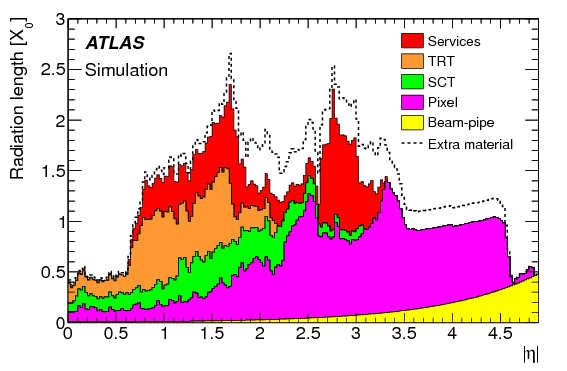
\includegraphics[width=0.7\textwidth]{./figures/invariant_mass_zee/material_budget.png}
	\caption{Materialbudget in Einheiten der Strahlungslänge~$\mathrm{X}_0$ in Abhängigkeit der Pseudorapidität~$\eta$ für die verschiedenen Detektorkomponenten in ATLAS \cite{electron_atlas}.} 
	\label{fig:material_budget}
\end{figure}
In Abbildung \ref{fig:material_budget} sieht man, dass das Materialbudget bei kleinen Pseudorapiditäten für die Strahlröhre und Pixeldetektoren in der Größenordnung von \num{0.1} bis $\num{0.2} \, \mathrm{X}_0$ liegt.
Dies entspricht gemäß Gleichung \eqref{eq:radiation_length} einer Korrektur von etwa
\begin{align*}
	e^{\num{0.1}} \approx \SI{110}{\percent} \qquad \text{bis} \qquad e^{\num{0.2}} \approx \SI{120}{\percent}
\end{align*}
auf die berechneten Impulse je nach Pseudorapidität des betrachteten Elektrons.
Die invariante Masse bedarf einer Korrektur die in derselben Größenordnung liegt und ist dann ungefähr konsistent mit der realen Z-Masse von \SI{91.2}{\GeV}.


\section{Kalibration der Elektronen}

Für die weitere Durchführung des Versuchs ist es nötig, die Energiemessung durch das elektromagnetische Kalorimeter zu kalibrieren.
Da einerseits das Kalorimeter aus vielen unabhängigen Modulen besteht und andererseits die Elektronen im inneren Detektor Energie verlieren oder in einen nicht-sensitiven Bereich des Kalorimeters eintreten, kommt es zu systematischen Abweichungen in der Energiemessung.
Aus diesem Grund muss in einem ersten Schritt eine Energiekalibration des gesamten Detektors durchgeführt werden, wobei sowohl Position der Elektronen im Detektor als auch deren Energie berücksichtigt werden sollten.

Hierzu kommt ein Datensatz mit Zerfällen $\mathrm{Z}^0 \rightarrow \mathrm{e}^+ + \mathrm{e}^-$ zum Einsatz, da die Masse und Zerfallsbreite des $\mathrm{Z}^0$ sehr genau vermessen wurde und somit ein bekanntes Signal für die Kalibration liefert.
Dabei wird die Verteilung der gemessenen invarianten Elektron-Positron-Massen in guter Näherung durch eine Faltung einer nicht-relativistische Breit-Wigner-Funktion und einer Gauss-Funktion beschrieben.
Die Gauss-Funktion parametrisiert dabei die näherungsweise als gaußförmig angenommene Verzerrung aufgrund der begrenzten Detektorauflösung.
Darüber hinaus wird der Untergrund in diesem Prozess durch vier zusätzliche Parameter beschrieben.

Bei der Kalibration wird ein Fit-Objekt, welches durch das Analysepaket ROOT zur Verfügung gestellt wird, verwendet.
Dieses ermöglicht eine $\chi^2$-Anpassung der durch den Detektor gemessenen invarianten  Elektron-Positron-Massenverteilung an die oben genannte Anpassungshypothese.
Die Anpassung liefert dann die invariante Masse des $\mathrm{Z}^0$ sowie dessen natürliche Zerfallsbreite, die Verbreiterung aufgrund der Detektorauflösung, die vier Parameter des Untergrunds und die Normierung von Untergrund und Signal.

\subsection{Darstellung kinematischer Variablen des Zerfalls $\mathrm{Z}^0 \rightarrow \mathrm{e}^- + \mathrm{e}^+$}

Zunächst werden mit dem Befehl \texttt{tree->Draw()} Histogramme der Elektronen- bzw Positronenenergie sowie der invarianten Masse des Elektron-Positron-Paares erstellt.
Diese sind in der Abbildungen \ref{fig:kinematische_variablen} aufgetragen.

Wie für den symmetrischen Zerfall erwartet, sind die Energieverteilungen von Elektron und Positron identisch.
Diese zeigen ein Maximum, welches ungefähr bei der halben $\mathrm{Z}^0$-Masse liegt, wie es gemäß Abschnitt~\ref{sssec:kinamtik_zweikoerperzerfall} für hoch-energetische Elektronen zu erwarten ist.
Ein weiteres Merkmal der Verteilung ist der starke Abfall in der Elektronenzahl bei einer Energie von etwa \SI{10}{\GeV}, welcher dadurch zu erklären ist, dass an die Daten die Schnittbedingung gestellt wurde, dass die invariante Elektron-Positron-Masse größer sein muss als \SI{20}{\GeV}.

Das Maximum der invarianten Elektron-Positron-Masse liegt bereits wie erwartet in der Größenordnung der $Z^0$-Masse.
Eine quantitative Aussage über die Lage des Z-Peaks liefert der Aufruf der Fit-Methode auf die unkalibrierten Daten, was in Abbildung \ref{fig:uncalibrated} dargestellt ist.

Man sieht, dass die Anpassung eine $\mathrm{Z}^0$-Masse von \SI{85.8}{\GeV} sowie eine Detektorauflösung von \SI{5.816 +- 0.047}{\GeV} liefert.
Im Folgenden ist es die Aufgabe, durch eine Kalibration die Auflösung zu verbessern und die systematische Unterschätzung der $\mathrm{Z}^0$-Masse zu korrigieren.

\begin{figure}[htb]
	\centering
	\begin{overpic}[width=\textwidth,tics=10]{./data/root/calibration/new/uncalibrated.pdf}
		\put (43,1) {$m_\mathrm{inv}$ / \si{GeV}}
		\put (1,29) {\rotatebox{90}{Ereignisse}}
	\end{overpic}
	\caption{Histogramm der invarianten Elektron-Positron-Masse des Zerfalls $\mathrm{Z}^0 \rightarrow \mathrm{e}^- + \mathrm{e}^+$ mit unkalibrierten Daten. 
	Außerdem wurde mithilfe des ROOT-Fit-Objektes eine Anpassung an das Signal durchgeführt. Die so bestimmte Z-Masse beträgt \SI{85.8}{\GeV}.}
	\label{fig:uncalibrated}
\end{figure}

\begin{figure}[p]
	\centering
	\begin{subfigure}{\textwidth}
		\centering
		\begin{overpic}[width=.7\textwidth,tics=10]{./data/root/calibration/new/el_energy.pdf}
			\put (43,0) {\small $E_\mathrm{e^-}$ / \si{GeV}}
			\put (0,29) {\rotatebox{90}{\small Ereignisse}}
		\end{overpic}
		\subcaption{Verteilung der Elektronen-Energie.}
		\label{fig:el_energy}
	\end{subfigure}
	\begin{subfigure}{\textwidth}
		\centering
		\begin{overpic}[width=.7\textwidth,tics=10]{./data/root/calibration/new/pos_energy.pdf}
			\put (43,0) {\small $E_\mathrm{e^+}$ / \si{GeV}}
			\put (0,29) {\rotatebox{90}{\small Ereignisse}}
		\end{overpic}
		\subcaption{Verteilung der Positronen-Energie.}
		\label{fig:pos_energy}
	\end{subfigure}
	\begin{subfigure}{\textwidth}
		\centering
		\begin{overpic}[width=.7\textwidth,tics=10]{./data/root/calibration/new/inv_mass.pdf}
			\put (43,0) {\small $m_\mathrm{inv}$ / \si{GeV}}
			\put (0,29) {\rotatebox{90}{\small Ereignisse}}
		\end{overpic}
		\subcaption{Verteilung der invariante Masse des Elektron-Positron-Paars. Der Untergrund des Prozesses ist deutlich an der linken Flanke zu erkennen.}
		\label{fig:inv_masse}
	\end{subfigure}
	\caption{Darstellung einiger kinematischen Variablen im Datensatz mit $\mathrm{Z}^0 \rightarrow \mathrm{e}^- + \mathrm{e}^+$ Zerfällen.}
	\label{fig:kinematische_variablen}
\end{figure}


\subsection{Kalibration der Elektronen-Energie}

Wie bereits im vorigen Abschnitt erwähnt, zeigt Abbildung \ref{fig:uncalibrated} die Anpassung an die unkalibrierten Daten für die invariante Leptonen-Masse.
Diese zeigt sowohl eine systematische Abweichung von der tatsächlichen Z-Masse, als auch eine Verbreiterung des Signals durch die Detektorauflösung von \SI{5.816+-0.047}{\GeV}.
Das Ziel dieser Aufgabe ist es nun, die Detektorauflösung zu verbessern, sowie die systematischen Abweichungen zu eliminieren.
Dazu gilt es zunächst die Quelle der systematischen Abweichungen und die damit zusammenhängenden kinematischen Variablen der Leptonen zu identifizieren:
\begin{itemize}
	\item Azimuthalwinkel~$\phi$:
		Das Kalorimeter besteht aus unabhängigen Modulen, die in der Sensitivität variieren können.
		Dies hat einen systematischen Einfluss auf die Elektronen, die unter einem gewissen Azimuthalwinkel in eines der Kalorimeter eintreten.		
	
	\item Pseudorapidität~$\eta$:
		Auch die Pseudorapidität als Maß für den Polarwinkel unter dem die Elektronen in die Kalorimeter eintreten, ist sensitiv auf systematische Abweichungen der einzelnen Kalorimeter-Module.
		Darüber hinaus ist die Materialmenge, die von Teilchen im inneren Detektor durchlaufen werden muss, stark vom Polarwinkel abhängig. Dies wurde zuvor in Abbildung \ref{fig:material_budget} dargestellt.
		
	\item Energie~$E$:
		Letztlich zeigt der Energieverlust von hoch-energetischen Elektronen in Materie, welcher hauptsächlich durch Bremsstrahlung verursacht wird, eine starke Abhängigkeit von deren Energie.
		Daher muss eine zusätzliche Kalibration die Leptonen-Energie berücksichtigen.
\end{itemize}
Zur Kalibration wird ein iterativer Ansatz gewählt, bei dem die invariante Lepton-Masse für verschiedene Parameterbereiche der Elektronen dargestellt und die Verteilungsfunktion angepasst wird.
Ausgehend von der so bestimmten Masse des Z-Bosons wird das Energiesignal mit einem Faktor multipliziert, um für den gewählten Parameterbereich den tatsächlichen Wert der Z-Masse zu erreichen.
Die Kalibration wird durch C-Code in der Datei \texttt{ElecCalib.C} implementiert und ist in Anhang \ref{sec:quellcode_kalibration} komplett aufgeführt.

Dieses Vorgehen wurde, um die Abhängigkeiten untereinander zu minimieren, abwechselnd für die Parameter $\phi$, $\eta$ und die Elektronenenergie dreimal wiederholt.
Durch Beobachtung der Verteilung in den verschiedenen Parameterbereichen konnte nach dieser Kalibration keine signifikante systematische Abweichung mehr festgestellt werden.
Der angepasste Parameter für die Detektorauflösung wurde somit von anfänglich \SI{5.8}{GeV} auf \SI{3.0}{GeV} reduziert.
Im Anschluss wurde die gesamte Verteilung so kalibriert, dass der Schwerpunkt des Peaks mit der tatsächlichen Z-Masse von \SI{91,19+-0,01}{GeV} \cite{pdg} zusammenfällt.
Die invariante Leptonen-Masse für die abgeschlossene Kalibration ist in Abbildung \ref{fig:final_calibration} gezeigt.
\begin{figure}[htbp]
	\centering
	\begin{overpic}[width=\textwidth,tics=10]{./data/root/calibration/new/calibrated.pdf}
		\put (43,1) {$m_\mathrm{inv}$ / \si{GeV}}
		\put (1,29) {\rotatebox{90}{Ereignisse}}
	\end{overpic}
	\caption{Invariante Leptonen-Masse in $\mathrm{Z}^0 \rightarrow \mathrm{e}^- + \mathrm{e}^+$ nach Kalibration der Energiemessung.}
	\label{fig:final_calibration}
\end{figure}

\section{Messung der W-Boson-Masse}

Nachdem die elektromagnetischen Kalorimeter kalibriert wurden, kann eine Bestimmung der Masse des W-Bosons anhand eines Datensatzes mit Ereignissen $\mathrm{W} \rightarrow \ell + \nu$ erfolgen.
Konkret stehen mehrere Datensätze zur Verfügung deren Verwendung kurz erläutert werden soll:
\begin{itemize}
	\item ATLAS $\mathrm{W} \rightarrow \mathrm{e} + \nu$:
		Simulierte Daten des Zerfalls, welche zur Bestimmung der W-Masse genutzt werden.
		Dieser Datensatz steht mit kalibrierten und unkalibrierten Energien zur Verfügung, um den Einfluss der Kalibration aus dem vorigen Versuchsteil quantifizieren zu können.
	
	\item ATLAS $\mathrm{Z} \rightarrow \mathrm{e}^- + \mathrm{e}^+$:
		Simulierte Daten die zur Abschätzung der systematischen Fehler bei der Bestimmung der W-Masse genutzt werden, da die Masse des Z-Bosons sehr genau bekannt ist.
		
	\item Monte-Carlo Untergrund:
		Monte-Carlo Simulation des Untergrund von $\mathrm{W} \rightarrow \mathrm{e} + \nu$, welcher durch die Wahl geeigneter Schnittselektionen minimiert werden muss.
	
	\item Monte-Carlo $\mathrm{W} \rightarrow \mathrm{e} + \nu$:
		Monte-Carlo Simulation des Zerfalls für verschiedene W-Massen zur Erstellung einer Eichkurve um die W-Masse aus dem ATLAS Datensatz zu rekonstruieren.	
\end{itemize}
Im Folgenden soll zunächst ein Überblick über die Datensätze geschaffen werden und anschließend eine Bestimmung der W-Masse anhand der vorliegenden Daten erfolgen.

\subsection{Vergleich von ATLAS und MC-Datensätze}
Für diesen Vergleich betrachten wir den ATLAS Datensatz $\mathrm{W} \rightarrow \mathrm{e} + \nu$ mit kalibrierten Energien und einen der fünf Monte-Carlo Datensätze (mit simulierter W-Masse~$M_\mathrm{W} = \SI{80.5}{\GeV}$).
Um einen Überblick über die Datensätze zu gewinnen, wurden verschiedene Observablen (Jet-Anzahl, Transversalimpuls des Elektrons und des W-Bosons) in den Abbildungen \ref{fig:observablen_pt1} und \ref{fig:observablen_pt2} zusammengestellt.    \begin{sidewaysfigure}[h]
	\centering
	\begin{subfigure}{.49\textwidth}
		\centering
		\begin{overpic}[width=.7\textwidth,tics=10]{./data/root/wmass/exercise1/ATLAS_njet}
			\put (40,1) {\scriptsize Anzahl Jets}
			\put (2,25) {\rotatebox{90}{\scriptsize Ereignisse}}
		\end{overpic}
		\caption{Anzahl der Jets pro Ereignis~\texttt{njet} für die kalibrierten ATLAS Daten.}
		\label{fig:atlas_njet}
	\end{subfigure}
	\begin{subfigure}{.49\textwidth}
		\centering
		\begin{overpic}[width=.7\textwidth,tics=10]{./data/root/wmass/exercise1/MC_njet}
			\put (40,1) {\scriptsize Anzahl Jets}
			\put (3,25) {\rotatebox{90}{\scriptsize Ereignisse}}
		\end{overpic}
		\caption{Anzahl der Jets pro Ereignis~\texttt{njet} für die Monte-Carlo Daten.}
	\end{subfigure}
	\begin{subfigure}{.49\textwidth}
		\centering
		\begin{overpic}[width=.7\textwidth,tics=10]{./data/root/wmass/exercise1/ATLAS_el_pt}
			\put (17,1) {\scriptsize Transversalimpuls $p_\mathrm{T}$ des Elektrons / \si{GeV}}
			\put (1,25) {\rotatebox{90}{\scriptsize Ereignisse}}
		\end{overpic}
		\caption{Transversaler Elektronenimpuls~\texttt{el\_pt} für die kalibrierten ATLAS Daten.}
	\end{subfigure}
	\begin{subfigure}{.49\textwidth}
		\centering
		\begin{overpic}[width=.7\textwidth,tics=10]{./data/root/wmass/exercise1/MC_el_pt}
			\put (17,1) {\scriptsize Transversalimpuls $p_\mathrm{T}$ des Elektrons / \si{GeV}}
			\put (1,25) {\rotatebox{90}{\scriptsize Ereignisse}}
		\end{overpic}
		\caption{Transversaler Elektronenimpuls~\texttt{el\_pt} für die Monte-Carlo Daten.}
	\end{subfigure}
	\caption{Jet-Anzahl und transversaler Elektronenimpuls für kalibrierte ATLAS Daten von $\mathrm{W} \rightarrow e + \nu$ Zerfällen bzw.\ Monte-Carlo Daten mit einer simulierten W-Masse von \SI{80,5}{GeV}.}
	\label{fig:observablen_pt1}
\end{sidewaysfigure}
\begin{sidewaysfigure}[h]
	\centering
	\begin{subfigure}{.49\textwidth}
		\begin{overpic}[width=\textwidth,tics=10]{./data/root/wmass/exercise1/ATLAS_ptw}
			\put (20,1) {\small Transversalimpuls $p_\mathrm{T}$ des W-Bosons / \si{GeV}}
			\put (1,25) {\rotatebox{90}{\small Ereignisse}}
		\end{overpic}
		\caption{Transversaler $W$-Boson Impuls \texttt{ptw} für die kalibrierten ATLAS Daten.}
	\end{subfigure}
	\begin{subfigure}{.49\textwidth}
		\begin{overpic}[width=\textwidth,tics=10]{./data/root/wmass/exercise1/MC_ptw}
			\put (20,1) {\small Transversalimpuls $p_\mathrm{T}$ des W-Bosons / \si{GeV}}
			\put (1,25) {\rotatebox{90}{\small Ereignisse}}
		\end{overpic}
		\caption{Transversaler $W$-Boson Impuls \texttt{ptw} für die Monte-Carlo Daten.}
		\label{fig:mc_ptw}
	\end{subfigure}
	\caption{Transversaler Impuls des W-Bosons für kalibrierte ATLAS Daten von $\mathrm{W} \rightarrow e + \nu$ Zerfällen bzw.\  Monte-Carlo Daten mit einer simulierten W-Masse von \SI{80,5}{GeV}.}
	\label{fig:observablen_pt2}
\end{sidewaysfigure}

Sowohl im simulierten Monte-Carlo als auch im ATLAS-Datensatzes ist klar zu erkennen, dass die Anzahl der Jets ein Maximum bei 0 Jets pro Ereignis aufweist, sodass etwa die Hälfte aller Ereignisse keine Jets im Endzustand aufweisen.
Diese Jets können durch Gluon-Abstrahlung im Anfangs- oder Endzustand entstehen, welche folglich zu Jets hadronisieren.
Dennoch unterscheiden sich die ATLAS- und Monte-Carlo-Daten dahingehend, dass die Anzahl der Ereignisse mit steigender Jetanzahl~\texttt{njet} im MC-Datensatz wesentlich stärker abnimmt.

Darüber hinaus wurde in den Abbildungen der transversale Impuls des Elektrons~$p_\mathrm{T}$ für die Datensätze aufgetragen.
Diese weichen von der theoretisch erwarteten Verteilung aus Gleichung \eqref{eq:pt_spektrum} ab, da bei einer Messung nur eine endliche Detektorauflösung realisierbar ist und außerdem das W-Boson nicht immer ruhend erzeugt wird, wie es von der Gleichung vorausgesetzt wird.
Dennoch liegen die Maxima beider Verteilung in der Größenordnung der halben W-Masse und können nach einer geeigneten Schnittselektion für die Bestimmung der W-Masse genutzt werden.
Ein weiterer Unterschied ist die Form der linken Flanke der Verteilung, welche vermutlich darauf zurückzuführen ist, dass bei beiden Datensätzen zuvor unterschiedliche Schnittselektionen durchgeführt wurden.

Weiterhin ist in den Abbildungen der transversale Impulse des W-Bosons~\texttt{ptw} aufgetragen.
Man erkennt in beiden Datensätze, dass die W-Bosonen ein ausgeprägtes Maximum des transversalen Impulses bei kleinen Impulsen aufweisen.
Für diese Bosonen ist die Abweichung von dem in der Theorie erwarteten Spektrum in Gleichung \eqref{eq:pt_spektrum} am geringsten.
Ein signifikanter Unterschied ist, dass der ATLAS-Datensatz wesentlich mehr Bosonen mit hohen Impulsen aufweist, was auf die zuvor diskutierte Jetanzahl pro Ereignis zurückzuführen ist, jedoch erst im nächsten Abschnitt näher diskutiert werden soll.

\clearpage
\subsection{Transversales Impulsspektrum des W-Bosons}
\label{ssec:ptw_spektrum}

Im Anschluss wird das Spektrum des Transversalimpulses des W-Bosons in Abhängigkeit von der Anzahl Jets betrachtet, um für die Bestimmung der W-Masse eine geeignete Schnittselektion durchführen zu können.
Die Darstellung für Ereignisse ohne Jets ist in Abbildung \ref{fig:njet0} gezeigt, alle weiteren folgen in Abbildung \ref{fig:njet1-4}.
\begin{figure}[h]
	\centering
	\begin{overpic}[width=\textwidth,tics=10]{./data/root/wmass/exercise2/njet0}
		\put (25,1) {Transversalimpuls $p_\mathrm{T}$ des W-Bosons / \si{GeV}}
		\put (1,29) {\rotatebox{90}{Ereignisse}}
	\end{overpic}
	\caption{Transversaler Impuls des W-Bosons für Ereignisse ohne Jets.}
	\label{fig:njet0}
\end{figure}
\begin{sidewaysfigure}[h]
	\centering
	\begin{subfigure}{.49\textwidth}
		\centering
		\begin{overpic}[width=.7\textwidth,tics=10]{./data/root/wmass/exercise2/njet1}
			\put (15,1) {\scriptsize Transversalimpuls $p_\mathrm{T}$ des W-Bosons / \si{GeV}}
			\put (1,26) {\rotatebox{90}{\scriptsize Ereignisse}}
		\end{overpic}
		\caption{Ein Jet}
	\end{subfigure}
	\begin{subfigure}{.49\textwidth}
		\centering
		\begin{overpic}[width=.7\textwidth,tics=10]{./data/root/wmass/exercise2/njet2}
			\put (15,1) {\scriptsize Transversalimpuls $p_\mathrm{T}$ des W-Bosons / \si{GeV}}
			\put (1,26) {\rotatebox{90}{\scriptsize Ereignisse}}
		\end{overpic}
		\caption{Zwei Jets}
	\end{subfigure}
	\begin{subfigure}{.49\textwidth}
		\centering
		\begin{overpic}[width=.7\textwidth,tics=10]{./data/root/wmass/exercise2/njet3}
			\put (15,1) {\scriptsize Transversalimpuls $p_\mathrm{T}$ des W-Bosons / \si{GeV}}
			\put (1,26) {\rotatebox{90}{\scriptsize Ereignisse}}
		\end{overpic}
		\caption{Drei Jets}
	\end{subfigure}
	\begin{subfigure}{.49\textwidth}
		\centering
		\begin{overpic}[width=.7\textwidth,tics=10]{./data/root/wmass/exercise2/njet4}
			\put (15,1) {\scriptsize Transversalimpuls $p_\mathrm{T}$ des W-Bosons / \si{GeV}}
			\put (1,26) {\rotatebox{90}{\scriptsize Ereignisse}}
		\end{overpic}
		\caption{Vier Jets}
	\end{subfigure}
	\caption{Transversaler Impuls des W-Bosons für Ereignisse mit ein, zwei, drei oder vier Jets im Endzustand.}
	\label{fig:njet1-4}
\end{sidewaysfigure}
Für Ereignisse ohne Jets ist in Abbildung \ref{fig:njet0} deutlich zu erkennen, dass Zerfälle mit kleinem transversalen Impuls des W-Bosons bevorzugt sind.
Für eine Kollision von zwei Partonen ohne transversalen Impuls ist es notwendig, dass das W-Boson ebenfalls ohne transversalen Impuls erzeugt wird.
Da die Partonen in Hadronen-Kollisionen jedoch einen kleinen transversalen Impuls haben können, zeigt sich in Abbildung \ref{fig:njet0}, dass in realen Kollisionen das Boson stehts mit einem nicht-ver\-schwin\-den\-den (jedoch kleinen) transversalen Impuls erzeugt wird.

Zusätzliche Jets in den $\mathrm{W} \rightarrow \mathrm{e} + \nu$ Ereignissen können durch Abstrahlung von Gluonen im Anfangs- oder Endzustand entstehen.
Dadurch wird die Viererimpuls-Bilanz verändert und das W-Boson muss mit einem signifikanten transversalen Impuls erzeugt werden.
In der Abbildung \ref{fig:njet1-4} wurde das transversale Impulsspektrum des W-Bosons für verschiedene Jet-Anzahlen im Endzustand dargestellt.
Es ist deutlich zu erkennen, dass der transversale Impuls des W-Bosons mit steigender Anzahl von Jets im Endzustand zunimmt, wie es aufgrund der Viererimpuls-Erhaltung erforderlich ist.

Dieser Effekt führt auch zu der Abweichung in Abbildung \ref{fig:observablen_pt2} für höhere transversale Impulse, da der ATLAS-Datensatz wesentlich mehr Ereignisse mit hohen Jet-Anzahlen aufweist als der Monte-Carlo-Datensatz (vgl.\ Abbildung \ref{fig:observablen_pt1})


\clearpage
\subsection{Schnittselektion der Ereignisse}
\label{ssec:schnittselektion}
Um die zur Verfügung stehenden Daten für eine aussagekräftige Messung zu verwenden, werden die Daten durch Schnittselektionen reduziert.
Hierzu werden Ereignisse mit W-Bosonen ausgewählt, die beinahe als ruhend angenommen werden können, so dass nur solche mit Transversalpimpuls $p_\mathrm{T}<\SI{12}{GeV}$ zur Auswertung betrachtet werden.
Der Grund für diese Selektion ist, dass aufgrund von Abschnitt \ref{sssec:kinamtik_zweikoerperzerfall} kleine Transversalimpulse des Bosons zu geringeren Verbreiterung des Jakobi-Maximums führen und so eine bessere Bestimmung der Masse ermöglichen sollten.
Für den Zerfall wird dann erwartet, dass geladenes Lepton und Neutrino beide einen Impuls in der Größenordnung der halben W-Masse tragen, der aufgrund ihrer geringen Masse gleich ihrer Energie gesetzt werden kann.
Dadurch lässt sich der erwartete Energiebereich der Leptonen einschränken.
Es wurde eine Schnittbedingung für den transversalen Elektronenimpuls und die fehlende transversale Energie $\slashed{E}_\mathrm{T}$, die als Impuls des Neutrinos aufgefasst werden kann die Schnittbedingungen $p_\mathrm{T,e}>\SI{25}{Gev}$ und $\slashed{E}_\mathrm{T}>\SI{25}{Gev}$ formuliert.
Aufgrund der erwarteten Elektronenenergie kann mit der Schnittbedingung $E_\mathrm{e}<\SI{65}{GeV}$ eine obere Grenze gesetzt werden.
Die verbleibende Einschränkung, nur Ereignisse mit weniger als \num{2} Jets zu berücksichtigen stellt sich als redundant heraus, da beinahe keine Ereignisse mit \num{2} Jets oder mehr in den selektierten Daten zu finden sind, wie nach Formulierung der Selektion festgestellt wurde.
Dies ist auf den Schnitt des Transversalimpulses des W-Bosons zurückzuführen, da gemäß Abschnitt \ref{ssec:ptw_spektrum} der transversale Impuls des Bosons für geringe Jet-Anzahlen im Endzustand klein ist.

Die selektierten Daten sind als Histogramm des Bosonimpulses in Abbildung \ref{fig:selektion_final} dargestellt.
\begin{figure}[htbp]
	\centering
	\begin{overpic}[width=\textwidth,tics=10]{./data/root/wmass/exercise3/ATLAS_cut}
		\put (26,1) {Transversalimpuls $p_\mathrm{T}$ des Elektrons / \si{GeV}}
		\put (1,29) {\rotatebox{90}{Ereignisse}}
	\end{overpic}
	\caption{Nach Anwenden der Selektion verbleibende Daten als Histogramm des transversalen Impulses des W-Bosons.}
	\label{fig:selektion_final}
\end{figure}
Eine Schwierigkeit stellte dar, die Schnitte so zu wählen, dass nicht relevante Ereignisse nicht berücksichtigt werden, aber genügend viele Ereignisse für eine aussagekräftige Statistik erhalten bleiben.
Darüber hinaus sollen die Selektion den Untergrund weitgehend unterdrücken.
Dieser wird nach Anwendung der Schnittbedingung in Abbildung \ref{fig:mc_bg} dargestellt und zeigt, dass die Schnittselektion den Monte-Carlo Untergrund von 7121 auf 261 Ereignisse reduzieren kann, was einer Unterdrückung von etwa \SI{96}{\percent} entspricht. 
\begin{figure}[h]
	\centering
	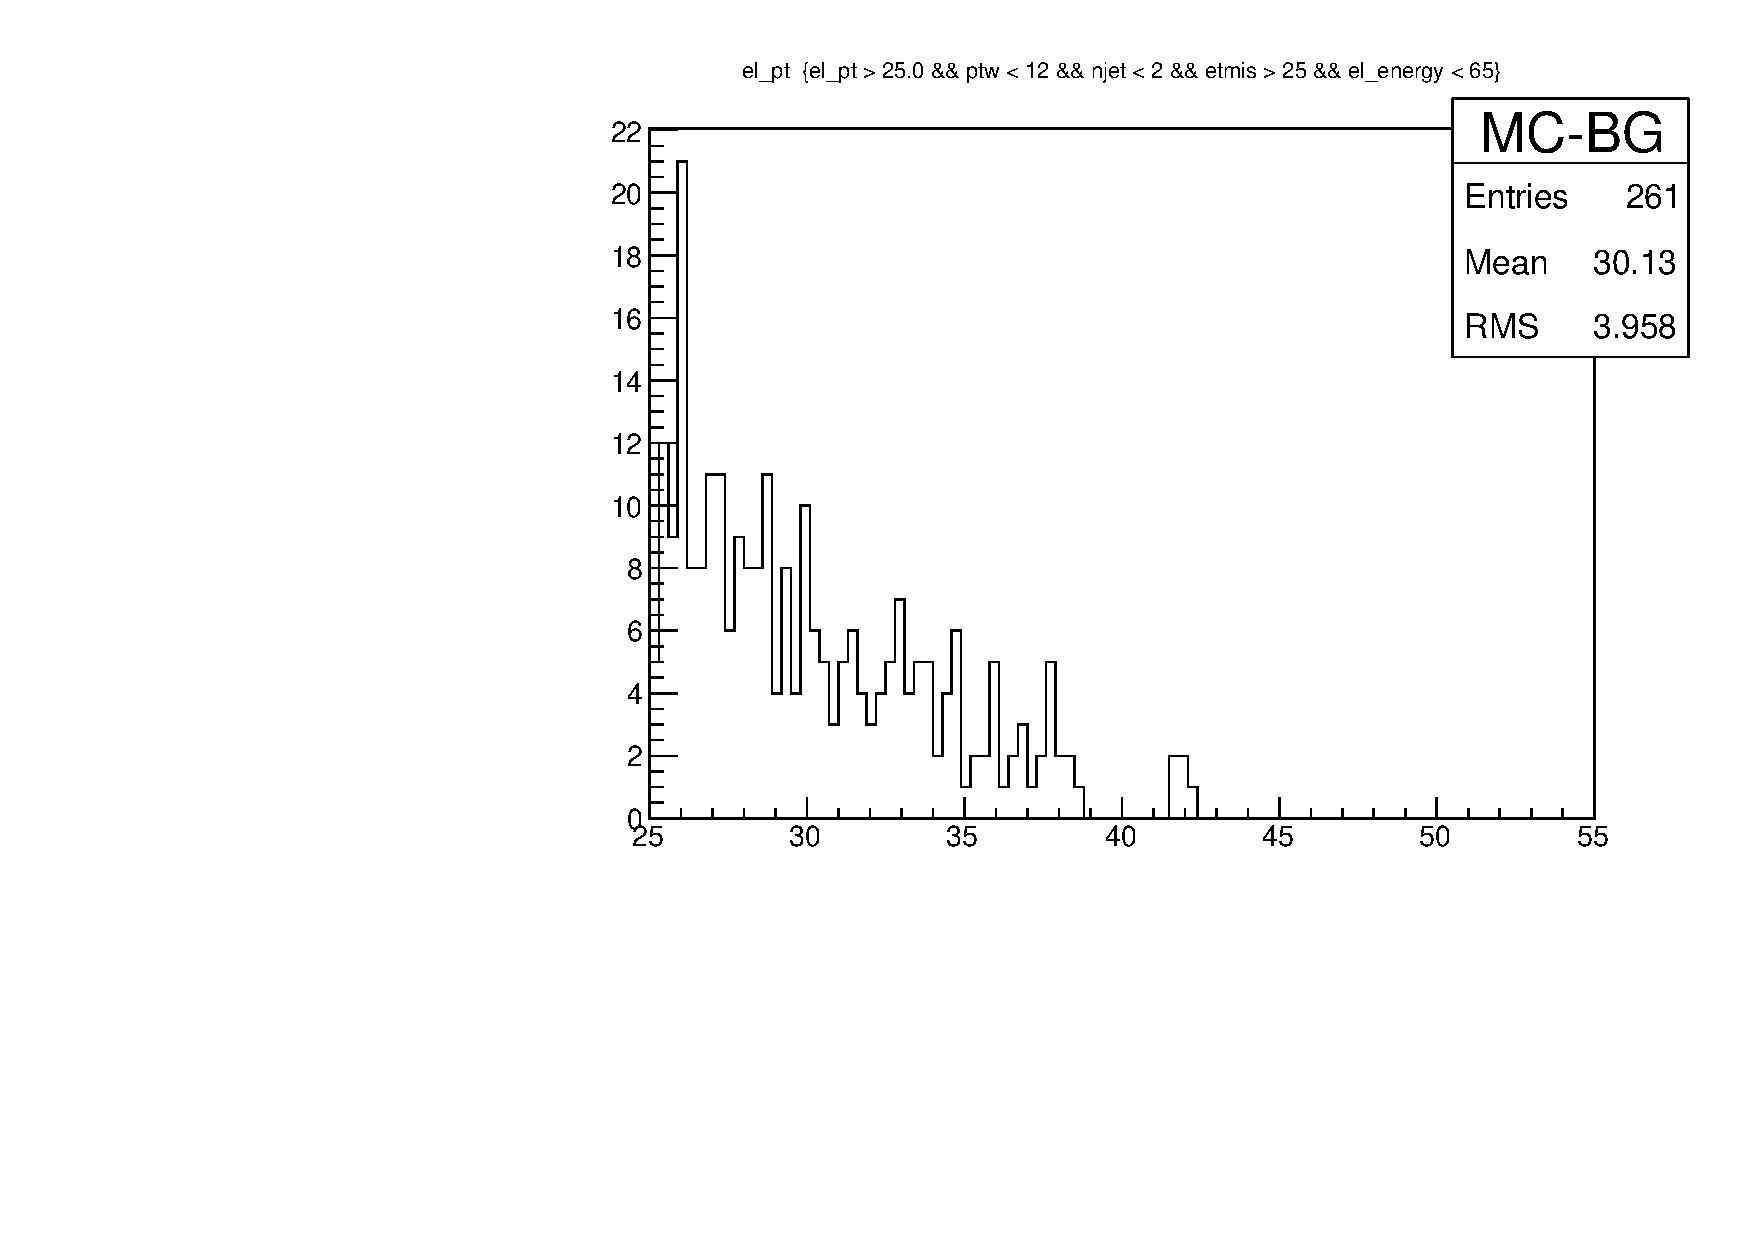
\includegraphics[width=1.0\textwidth]{./data/root/wmass/exercise4/mc_bg.pdf}
	\caption{Monte-Carlo-Simulation vom Untergrund des Prozesses $\mathrm{W} \rightarrow \mathrm{e} + \nu$ nach Anwendung der Schnittbedingung. Vor Anwendung der Schnittbedingung enthielt die Simulation 7121 Ereignisse.}
	\label{fig:mc_bg}
\end{figure}

\subsection{Bestimmung der Halbhöhenpunkte}
\label{sec:selektion}

Nachdem die Schnittselektion aufgestellt wurde und der Untergrund hinreichend unterdrückt wurde, kann diese auf die verfügbaren Datensätze angewendet werden.
Mithilfe einer Anpassungs-Methode des ROOT-Objektes können die Halbhöhenpunkte~$h$ der Transversalimpuls-Verteilung des Elektrons angepasst werden.
Eine solche Anpassung ist für die kalibrierten ATLAS-Daten in Abbildung \ref{fig:halbhöhe_atlas_calib} gezeigt, die angepassten Werte für alle Datensätze sind in Tabelle \ref{tab:halbhoehen} zu finden.
\begin{figure}[htbp]
	\centering
	\begin{overpic}[width=\textwidth,tics=10]{./data/root/wmass/exercise4/atlas_calib}
		\put (26,1) {Transversalimpuls $p_\mathrm{T}$ des Elektrons / \si{GeV}}
		\put (1,29) {\rotatebox{90}{Ereignisse}}
	\end{overpic}
	\caption{Anpassung der Verteilung an die Hypothese des ROOT-Fit-Objekts und Bestimmung des Halbhöhenpunktes $h$ für die kalibrierten ATLAS Daten des  $\mathrm{W} \rightarrow \mathrm{e} + \nu$ Zerfalls.}
	\label{fig:halbhöhe_atlas_calib}
\end{figure}
\begin{table}[htbp]
	\centering
	\begin{tabular}{lSS}
\toprule
Datensatz 									      & {Halbhöhenpunkt $h$ / \si{GeV}} & {$\sigma_h$ / \si{GeV}} \\
\midrule
Monte-Carlo ($m_\mathrm{W}=\SI{79,0}{\GeV}$)      & 41.00 &         0.10 \\
Monte-Carlo ($m_\mathrm{W}=\SI{79,5}{\GeV}$)      & 41.26 &         0.10 \\
Monte-Carlo ($m_\mathrm{W}=\SI{80,0}{\GeV}$)      & 41.48 &         0.08 \\
Monte-Carlo ($m_\mathrm{W}=\SI{80,5}{\GeV}$)      & 41.92 &         0.15 \\
Monte-Carlo ($m_\mathrm{W}=\SI{81,0}{\GeV}$)      & 41.97 &         0.09 \\
Monte-Carlo ($\mathrm{Z}\rightarrow e e$)         & 47.13 &         0.21 \\
Monte-Carlo Untergrund                            &       &              \\
ATLAS kalibriert ($\mathrm{W}\rightarrow e\nu$)   & 42.10 &         0.07 \\
ATLAS unkalibriert ($\mathrm{W}\rightarrow e\nu$) & 41.37 &         0.08 \\
ATLAS kalibriert ($\mathrm{Z}\rightarrow e e$)    & 47.54 &         0.26 \\
ATLAS unkalibriert ($\mathrm{Z}\rightarrow e e$)  & 47.19 &         0.26 \\
\bottomrule
\end{tabular}

	\caption{Angepasste Halbhöhenpunkte $h$ für die zur Verfügung stehenden Datensätze. Durch die Schnittselektion blieben zu wenig Ereignisse in dem Datensatz mit Monte-Carlo Untergrund übrig, so dass keine Anpassung erfolgen konnte.}
	\label{tab:halbhoehen}
\end{table}

Für die Datensätze $\mathrm{Z} \rightarrow ee$ musste die Schnittbedingung modifiziert werden, da im Z-Zerfall die Variable~\texttt{ptw} (Transversalimpuls des W-Bosons) undefiniert ist und keine Neutrinos auftreten, sodass keine signifikante fehlende transversale Energie~$\slashed{E}_\mathrm{T}$ festzustellen ist.
Aus diesem Grund wurde \texttt{ptw} durch den transversalen Impuls des Elektron-Positron-Paares~\texttt{pt\_ee} ersetzt, der dem transversalen Impuls des Z-Bosons entspricht.
Außerdem entfällt die Bedingung an fehlende transversale Energie~$\slashed{E}_\mathrm{T}$.

\subsection{Erstellung einer Eichkurve aus Monte-Carlo-Daten}
A priori ist nicht klar, ob der angepasste Halbhöhenpunktes~$h$ der Polstelle in Gleichung \eqref{eq:pt_spektrum} entspricht.
Aus diesem Grund ist ein direktes Ablesen der W-Masse mithilfe dieses Punktes nicht möglich.
Stattdessen werden die Monte-Carlo Daten mit verschiedenen simulierten W-Massen genutzt, um eine Eichkurve für die Masse zu erzeugen.

Zur Bestimmung der Eichkurve wird die simulierte W-Masse~$M_\mathrm{MC}$ gegen die durch ROOT angepasste Position des Halbhöhenpunktes~$h$ aufgetragen (vgl.\ Tabelle~\ref{tab:halbhoehen}) und eine Gerade an die Daten angepasst.
Um bei der Anpassung der Geraden die Fehler in der Halbhöhenpunkt-Messung korrekt zu beachten, wird diese durch eine orthogonale Regression \cite{odr} durchgeführt.
Als Anpassungshypothese wird
\begin{align*}
	M(h) = m \cdot h + b
\end{align*}
mit den Parametern $m$ und $b$ genutzt.
Das Ergebnis der Anpassung ist in Abbildung \ref{fig:gauge_curve} gezeigt.
\begin{figure}[h]
	\centering
	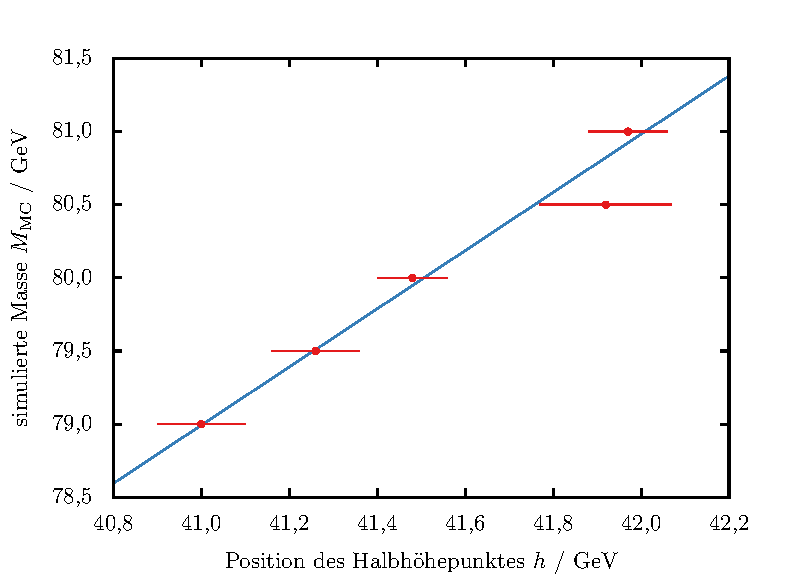
\includegraphics{./figures/wmass/gauge.pdf}
	\caption{Anpassung einer Eichkurve für die Masse des Bosons an die gemessenen Halbhöhenpunkte der Monte-Carlo-Simulationen aus Tabelle \ref{tab:halbhoehen}.}
	\label{fig:gauge_curve}
\end{figure}

\noindent Nach der Anpassung ergibt sich für die Parameter:
\begin{align*}
	m &= \num{1.990 +- 0.182} \\
	b &= \SI{-2.58 +- 7.54}{\GeV}
\end{align*}
mit einem reduzierten Chi-Quadrat von $\chi_\mathrm{red.}^2 = \num{0.638}$.
Daraus ist zu folgern, dass die Anpassungshypothese die vorliegenden Daten gut beschreibt, jedoch die Fehler durch die Anpassung von ROOT etwas überschätzt wurden.

Bei der Verwendung dieser angepassten Eichkurve muss beachtet werden, dass die Fehler von Steigung~$m$ und Achsenabschnitt~$b$ stark korreliert sind.
Dies wird durch die Kovarianzmatrix beschrieben wird, welche ebenfalls als Ergebnis der Anpassung vorliegt:
\begin{align*}
			\Sigma^\mathrm{Eichk.} &= \begin{pmatrix}
			\sigma_m^2 & \sigma_{mb} \\
			\sigma_{bm} & \sigma_b^2
			\end{pmatrix}\\
			&= \begin{pmatrix}
			\num{0.03306} & \num{-1.372} \\
			\num{-1.372}    & \num{56.93}
			\end{pmatrix} \, \text{.}\\
\end{align*}
Auf der Diagonalen dieser Matrix finden sich die Varianzen der einzelnen Anpassungsparameter und auf der Nebendiagonalen finden sich die Korrelationen der Fehler zwischen beiden Parametern.
Die konkrete Auswertung innerhalb der \textsc{Gauß}schen Fehlerfortpflanzung, sowie die Diskussion der systematischen Abweichungen und Korrekturen findet im nächsten Abschnitt statt.

\subsection{Bestimmung der W-Masse}
Abschließend soll mithilfe der aufgenommenen Daten eine Bestimmung der W-Masse durchgeführt werden.

\subsubsection{Korrektur der Massebestimmung}
\label{sssec:korrektur}
Zu einer Abweichung bei der Massebestimmung kommt es durch abweichende $p_\mathrm{T}$-Spektren der Elektronen in den ATLAS- sowie Monte-Carlo-Daten.
In dieser Hinsicht wurde bereits bei der Schnittselektion in Abschnitt~\ref{ssec:schnittselektion} sichergestellt, dass nach Anwendung der Schnitte auf die Datensätze ein ähnliches $p_\mathrm{T}$-Spektrum des Elektrons entsteht, sodass systematische Abweichungen vermieden werden können.
Ein Vergleich beider Spektren ist in Abbildung~\ref{fig:vgl_spektren} dargestellt, wobei die Anzahl der MC-Ereignisse auf die des ATLAS-Datensatzes hochskaliert wurde.
\begin{figure}[h]
	\centering
	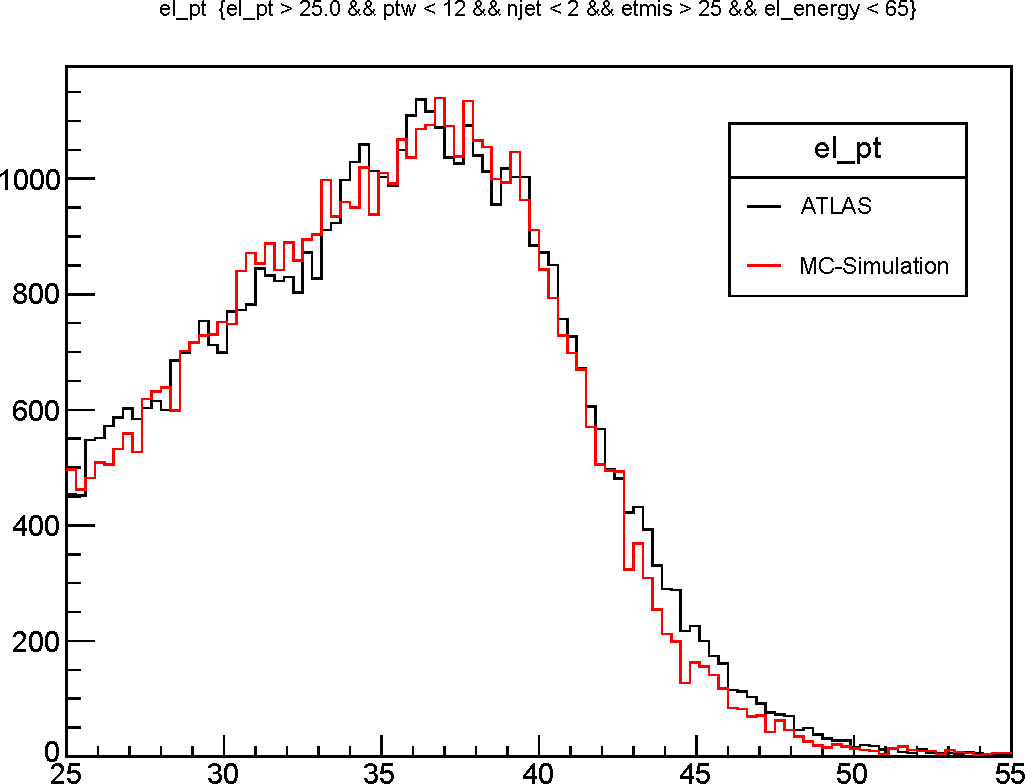
\includegraphics[width=.8\textwidth]{./figures/wmass/comparison.pdf}
	\caption{Vergleich der Spektren der transversalen Impulse für den ATLAS- und MC-Datensatz ($M_\mathrm{W} = \SI{80.5}{\GeV}$). \korr{Achsenbeschriftung}}
	\label{fig:vgl_spektren}
\end{figure}
In der Abbildung kann eine gute Übereinstimmung beider Spektren festgestellt werden.

Dennoch kann nicht direkt die Position des Halbhöhenpunktes aus dem ATLAS-Datensatz in die Eichkurve, die aus Monte-Carlo-Daten gewonnen wurde, eingesetzt werden.
Es ist folglich erforderlich, dass eine Umrechnung zwischen den Halbhöhenpunkten für die ATLAS-Daten~$h_\mathrm{ATLAS}$ und die Monte-Carlo-Daten~$h_\mathrm{MC}$ bestimmt wird.
Da die Z-Masse sehr genau bestimmt wurde, wird daher der kalibrierte ATLAS-Datensatz $\mathrm{Z} \rightarrow ee$ und die Monte-Carlo-Simulation desselben Zerfalls für diese Korrektur verwendet.
Eine Näherung erster Ordnung ist durch
\begin{align*}
	h_\mathrm{MC} = \frac{h_{\mathrm{Z, MC}}}{h_{\mathrm{Z, ATLAS}}} \cdot h_\mathrm{ATLAS}
\end{align*}
gegeben, wobei der Faktor aus den Werten der Tabelle~\ref{tab:halbhoehen} zu
\begin{align*}
	\frac{h_{\mathrm{Z, MC}}}{h_{\mathrm{Z, ATLAS}}} = \num{0.9914 +- 0.0070}
\end{align*}
bestimmt werden kann.


\subsubsection{Bestimmung der W-Masse}
In Abschnitt \ref{sec:selektion} wurde die Position des Halbhöhenpunktes~$h$ für die simulierten und kalibrierten ATLAS-Daten zu
\begin{align*}
	h_\mathrm{ATLAS} = \SI{42.10 +- 0.07}{\GeV}
\end{align*}
bestimmt.
Nach Anwendung der Korrektur aus Abschnitt~\ref{sssec:korrektur} erhält man:
\begin{align*}
	h = \SI{41.74 +- 0.30}{\GeV} \, \text{.}
\end{align*}
Um schließlich die W-Masse mithilfe der zuvor angepassten Eichkurve zu bestimmen, ist es nötig die gemeinsame Kovarianzmatrix für die Kurvenparameter $m, b$ und des korrigierten Halbhöhenpunktes~$h$ zu bestimmen.
Da diese Fehler unabhängig sind, lässt sich die neue Kovarianzmatrix durch Bildung der Blockdiagonalmatrix
\begin{align*}
	\Sigma^\mathrm{tot} = \begin{pmatrix}
		\sigma_m^2  & \sigma_{mb} & 0 \\
		\sigma_{bm} & \sigma_b^2  & 0 \\
		0           & 0           & \sigma_h^2
	\end{pmatrix}
\end{align*}
erzeugen.
Außerdem wird für die Auswertung der Eichkurve $M(m, b, h)$ die Jakobi-Matrix
\begin{align*}
	J &= \begin{pmatrix}
	\frac{\partial M}{\partial m} &
	\frac{\partial M}{\partial b} &
	\frac{\partial M}{\partial h}
	\end{pmatrix} \\
\end{align*}
benötigt.
Mit der Eichkurve $M(m, b, h) = m \cdot h + b$ folgt die explizite Darstellung
\begin{align*}
	J=\begin{pmatrix}
	h & 1 & m
	\end{pmatrix} \, \text{.}
\end{align*}
Dadurch erhält man nach der Auswertung der Eichkurve durch Anwendung von \textsc{Gauß}scher Fehlerfortpflanzung gemäß \cite{error_prop}
\begin{align*}
	\Sigma^M = \begin{pmatrix}
	\sigma_{M}^2
	\end{pmatrix} = J \, \Sigma^\mathrm{tot} \, J^\mathrm{T}
\end{align*}
die $1 \times 1$ Kovarianzmatrix für die Masse~$M$ mit dem Standardfehler~$\sigma_M$.
Setzt man die Kurvenparameter und die Position des Halbhöhenpunktes sowie deren Fehler ein, so erhält man für die W-Masse
\begin{align*}
	M_\mathrm{W} = \SI{80.46 +- 0.60}{\GeV}
\end{align*}
Die Notwendigkeit der Beachtung der Fehlerkorrelationen wird hier klar, da alleine aufgrund des großen Fehlers auf dem Achsenabschnitt von etwa \SI{7}{\GeV} bei der naiven Fehlerfortpflanzung ohne Beachtung der Korrelationen ein Fehler in derselben Größenordnung zu erwarten ist.
Zum Vergleich ist der Literaturwert für die W-Masse \cite{pdg}
\begin{align*}
	M_\mathrm{W}^\mathrm{Lit.} = \SI{80.385 +- 0.015}{\GeV}
\end{align*}
und ist in Anbetracht der statistischen Fehler in guter Übereinstimmung mit dem in diesem Versuch bestimmten Wert.
Der Einfluss der Kalibration und etwaige systematische Fehler werden im nächsten Abschnitt untersucht.

\subsubsection{Einfluss der Kalibration und systematische Abweichungen}



\section{Fazit}

\FloatBarrier
% BIBLIOGRAPHIE
\vspace{\fill}
% Maximale Anzahl der Einträge in Klammer
% Zitieren mit \cite{lamport94}
\begin{thebibliography}{19}
\bibitem{script}
	N. Möser, J. Meier, J.-W. Tsung, E. von Törne,
	\emph{Der ATLAS-Versuch: Eigenschaften von W-Bosonen und die Suche nach neuer Physik}.
\bibitem{pdg}
	K.A. Olive \textit{et al.} (Particle Data Group),
	\emph{The Review of Particle Physics},
	Chin. Phys. C, \textbf{38}, 090001 (2014).

\bibitem{electron_atlas}
	ATLAS Collaboration (Aad, Georges \textit{et al.}),
	\emph{Electron performance measurements with the ATLAS detector using the 2010 LHC proton-proton collision data},
	Eur.\ Phys.\ J.\ C72 (2012) 1909.

\bibitem{odr}
	SciPy,
	\emph{Orthogonal distance regression (\texttt{scipy.odr})},
	\url{http://docs.scipy.org/doc/scipy/reference/odr.html} (Letzter Aufruf: 14. März 2016).

\bibitem{error_prop}
	B. Ochoa, S. Belongie,
	\emph{Covariance Propagation for Guided Matching},
	\url{http://vision.cornell.edu/se3/wp-content/uploads/2014/09/ochoa06.pdf} (Letzter Aufruf: 14. März 2016).
	
\bibitem{wiki_standardmodell}
	\emph{Wikimedia Commons, the free media repository}. \url{https://commons.wikimedia.org/wiki/File:Standard_Model_of_Elementary_Particles-de.svg} (Letzter Aufruf: 15. März 2016)
	
\bibitem{cern}
	CERN \emph{Computer generated image of the whole ATLAS detector (CERN-GE-0803012-06)}.\url{http://cds.cern.ch/record/1095924} (Letzter Aufruf: 15. März 2016)
\end{thebibliography}

% APPENDIX
\begin{appendix}
\newpage
\section{Anhang}
\subsection{Vorbereitungsaufgaben}

\subsubsection*{6.2.2 - Frage A}
Der Viererimpuls muss in der Reaktion erhalten sein, so dass man schreiben kann:
\begin{align*}
	\mathbf{p}_{\mathrm{Z}^0}^2=m_{\mathrm{Z}^0}^2&=(\mathbf{p}_{\mathrm{e}^-}+\mathbf{p}_{\mathrm{e}^+})^2\\
	&=2m^2_{\mathrm{e}} + 2 E_{\mathrm{e}^-} E_{\mathrm{e}^+} - 2\vec{p}_{\mathrm{e}^-}\vec{p}_{\mathrm{e}^+}
\end{align*}
Im Ruhesystem des $\mathrm{Z}^0$ gilt $\vec{p}_{\mathrm{e}^-}=-\vec{p}_{\mathrm{e}^+}$ und $E_{\mathrm{e}^-}=E_{\mathrm{e}^+}$. Daraus folgt:
\begin{align*}
	m_{\mathrm{Z}^0}^2&=2m^2_{\mathrm{e}} + 2 E_{\mathrm{e}}^2 + 2|\vec{p}_{\mathrm{e}}|^2
\end{align*}
Aus der Energie-Impuls-Beziehung $E=\sqrt{m^2+|\vec{p}|^2}$ folgt somit:
\begin{align*}
	m_{\mathrm{Z}^0}^2 - 4m^2_{\mathrm{e}} &= 4|\vec{p}_{\mathrm{e}}|^2\\
	|\vec{p}_{\mathrm{e}}|&=\sqrt{\frac{m_{\mathrm{Z}^0}^2 - 4m^2_{\mathrm{e}}}{4}} \approx \SI{45.6}{GeV}
\end{align*}

\subsubsection*{6.2.2 - Frage B}
Die Aufgabe erfolgt analog zu Frage A, jedoch mit der Schwerpunktsenergie von \SI{5}{GeV} anstatt $m_{\mathrm{Z}^0}$. Dann ergibt sich:
\begin{align*}
	|\vec{p}_{\mathrm{\tau}}|&=\sqrt{\frac{(\SI{5}{GeV})^2 - 4m^2_{\mathrm{\tau}}}{4}} \approx \SI{1.76}{GeV}
\end{align*}

\subsubsection*{6.3.1 - ptw}
Aufgrund der Impulserhaltung kann der Transversalimpuls des W-Bosons \texttt{ptw} aus den Messungen des transversalen Elektronimpulses und dem fehlenden transversalen Impuls (aufgrund des Neutrinos) bestimmt werden:
\begin{align*}
	p_\mathrm{T,W}=\sqrt{(p_\mathrm{e,x} + p_\mathrm{mis, x})^2 + (p_\mathrm{e,y} + p_\mathrm{mis, y})^2}
\end{align*}

\subsubsection*{6.3.1 - Herleitung}
\label{sssec:herleitung_jacobi}
Mit der Kettenregel folgt:
\begin{align*}
	\frac{\mathrm{d}\sigma}{\mathrm{d}p_\mathrm{T}} = \frac{\mathrm{d}\sigma}{\mathrm{d}\cos\vartheta^*}\left|\frac{\mathrm{d}\cos\vartheta^*}{\mathrm{d}p_\mathrm{T}}\right| = \frac{\mathrm{d}\sigma}{\mathrm{d}\cos\vartheta^*}\frac{1}{\left|\frac{\mathrm{d}p_\mathrm{T}}{\mathrm{d}\cos\vartheta^*}\right|}
\end{align*}
Es gilt $p_\mathrm{T}=p^*\sin\vartheta^*$ mit $p^*$ dem Impuls im Schwerpunktsystem, wobei für eine vernachlässigbar kleine Leptonmasse $p^*\approx\frac{1}{2}M_\mathrm{W}$ angenommen werden kann.
Dann gilt:
\begin{align*}
	\frac{\mathrm{d}p_\mathrm{T}}{\mathrm{d}\cos\vartheta^*}=p^*\frac{\mathrm{d}\sin\vartheta^*}{\mathrm{d}\cos\vartheta^*}=-p^*\frac{\cos\vartheta^*}{\sin\vartheta^*}
\end{align*}
Mit der Ableitung folgt für $\frac{\mathrm{d}\sigma}{\mathrm{d}p_\mathrm{T}}$:
\begin{align*}
	\frac{\mathrm{d}\sigma}{\mathrm{d}p_\mathrm{T}}&=\frac{\mathrm{d}\sigma}{\mathrm{d}\cos\vartheta^*} \frac{1}{p^*\left|\frac{\cos\vartheta^*}{\sin\vartheta^*}\right|}\\
	&=\frac{\mathrm{d}\sigma}{\mathrm{d}\cos\vartheta^*} \frac{1}{p^*\left|\frac{p^*\sqrt{1-\sin^2\vartheta^*}}{p^*\sin\vartheta^*}\right|}\\
	&=\frac{\mathrm{d}\sigma}{\mathrm{d}\cos\vartheta^*} \frac{1}{p^*\left|\frac{\sqrt{{p^*}^2-{p^*}^2\sin^2\vartheta^*}}{p^*\sin\vartheta^*}\right|}\\
	&=\frac{\mathrm{d}\sigma}{\mathrm{d}\cos\vartheta^*} \frac{1}{p^*\frac{\sqrt{{p^*}^2-p_\mathrm{T}^2}}{p_\mathrm{T}}}\\
	&=\frac{\mathrm{d}\sigma}{\mathrm{d}\cos\vartheta^*} \frac{p_\mathrm{T}}{p^*\sqrt{{p^*}^2-p_\mathrm{T}^2}}\\
	&\approx \frac{\mathrm{d}\sigma}{\mathrm{d}\cos\vartheta^*} \frac{2p_\mathrm{T}}{M_\mathrm{W}} \frac{1}{\sqrt{\frac{1}{4}M_\mathrm{W}^2-p_\mathrm{T}^2}}
\end{align*}
\subsubsection*{6.4.1 - 1.)}
Die invariante Vier-Lepton-Masse muss mindestens so groß sein wie $2m_\mathrm{Z^0}$, wenn die Z-Bosonen reell sind.
Der Minimalfall tritt genau dann ein, wenn die Z-Bosonen ruhend erzeugt werden.
Unterhalb dieser Schwelle können dennoch Zerfälle stattfinden, bei denen mindestens eines der Z-Bosonen virtuell auftritt.

\subsubsection*{6.4.1 - 2.)}
Man erwartet eine Breit-Wigner-Verteilung der invarianten Masse mit Maximum bei der Masse des Higgs-Bosons und einer charakteristischen Breite~$\Gamma$.

\subsubsection*{6.4.1 - 3.)}
In einem idealen Detektor würden sowohl Elektronen als auch Myonen sowie Jets vollständig detektiert werden, das heißt es findet eine ideale Energie- und Impulsmessung statt, so dass keine fehlende Energie auftritt.
Aufgrund der endlichen Auflösung eines realen Detektors tritt in diesem Fall eine geringe, aber von null verschiedene fehlende Energie auf.

\subsubsection*{6.4.1 - 4.)}
Die im $\mathrm{t}$-Zerfall auftretenden $\mathrm{b}$-Quarks hadronisieren zu Mesonen, die über die schwache Wechselwirkung zerfallen, wobei zusätzliche Leptonen im Endzustand erzeugt werden können.

\subsubsection*{6.4.1 - 5.)}
Der statistische Fehler auf die Anzahl Einträge in einem Bin ist $\sqrt{N}$ ($N$: Erwartungswert für die Anzahl der Einträge), in dem vorliegenden Fall also \num{10}.
Die Wahrscheinlichkeit, in einem Bin \num{130} Einträge zu finden entspricht damit einer Abweichung von $3\sigma$ vom Mittelwert, die durch eine Integration über die Wahrscheinlichkeitsdichte zu \SI{0.27}{\percent} $\approx \frac{1}{370}$ bestimmt werden kann.
Da dies für alle Bins gilt, ist der Erwartungswert, für eine Abweichung von $3\sigma$ in \num{200} Bins: $\frac{1}{370} \cdot 200 \approx \num{0.54}$.
Insgesamt lässt sich die Wahrscheinlichkeit $P$, in mindestens einem Bin eine Abweichung von $3\sigma$ zu finden, dann bestimmen aus der Wahrscheinlichkeit, in keinem Bin eine Abweichung zu finden:
\begin{align*}
	P = 1 - \left(1 - \frac{1}{370}\right)^{200} \approx \SI{42}{\percent}
\end{align*}

\clearpage
\subsection{Quellcode der verwendeten Kalibration}
\label{sec:quellcode_kalibration}
\lstinputlisting[language=C]{./data/root/calibration/ElecCalib.C}

\end{appendix}

\end{document}
